\documentclass{beamer}
\usepackage[utf8]{inputenc}
\usepackage[T1]{fontenc}
\usepackage[french]{babel}

\DeclareUnicodeCharacter{1D49}{\textsuperscript{e}}
\DeclareUnicodeCharacter{202F}{\,}
\DeclareUnicodeCharacter{00A9}{\textcopyright}

% Packages from the first set
\usepackage{textpos}
\usepackage{graphicx}
\usepackage{wrapfig}
\usepackage{tikz}
\usetikzlibrary{shapes.geometric,calc}
\usepackage{amsmath,amssymb}
\usepackage[framemethod=TikZ]{mdframed}
\usepackage{caption}
\usetheme{Boadilla}
\usecolortheme{default}
\usepackage{lmodern}
\usepackage{array}
\usepackage{pgfgantt}
\usepackage{pgf-umlsd}

\usepackage{listings}
\usepackage{listingsutf8}
\lstset{inputencoding=utf8,extendedchars=true}

% Packages from the second set
\usepackage{xcolor}
\usepackage{subcaption}
\usepackage{float}
\usepackage{algorithm}
\usepackage{algorithmic}
\usepackage{microtype}
%\usepackage[hidelinks,pdfencoding=auto]{hyperref}
\PassOptionsToPackage{hidelinks,pdfencoding=auto}{hyperref}


\title[Rapport Projet]{Présentation PFE : Analyse des composantes principales (ACP)}
\subtitle{Etudes theorique et pratique}
\author[HANFAOUI K. ]{HANFAOUI Karim\inst{1}}
\institute[FSBM]{\inst{1} FSBM — 3ᵉ année Licence SMA \\ \texttt{karim.hanfaoui-etu@etu.univh2c.ma} \\[2pt]}
\date[JUIN 2025]{Faculte des sciences de Ben M'Sick \\ — \\ Mars → Juin 2025}

\AtBeginSection[]{
  \begin{frame}
    \frametitle{Table of Contents}
    \tableofcontents[currentsection]
  \end{frame}
}

\begin{document}

\begin{frame}
  \titlepage
  \begin{textblock*}{8cm}(9cm,-8.2cm)
    
\includegraphics[height=1.2cm]{logo-fsbVF}
  \end{textblock*}
\end{frame}

\begin{frame}{Remerciements}
\begin{center}\textit{Chers membres du jury,}\end{center}

Je tiens à vous remercier sincèrement pour votre présence et votre attention lors de ma soutenance de projet de fin d’étude. Cet aboutissement n’aurait pas été possible sans votre soutien et vos conseils tout au long de cette aventure.

\vspace{0.2cm}

Je souhaite également remercier Pr. \textsc{Adnaoui} Khalid pour sa collaboration et son engagement dans ce projet, ainsi que pour sa patience à mon égard. \textit{Nous avons travaillé ensemble avec passion et détermination pour offrir un travail de qualité.}
\end{frame}

\section{Introduction Générale}

\begin{frame}{Introduction Générale}
L'Analyse des Composantes Principales (ACP) est une méthode statistique de réduction de dimensionnalité qui transforme des variables corrélées en un ensemble de composantes orthogonales maximisant la variance expliquée. Fondée sur l'algèbre linéaire et la théorie des matrices, elle permet d'extraire l'information essentielle tout en préservant la structure des données.
\end{frame}

\begin{frame}{Problématique}
  \begin{alertblock}{Problématique}
    Comment peut-on réduire la dimension d’un ensemble de données représenté sous forme de matrice tout en conservant le maximum possible d’information ?
  \end{alertblock}
\end{frame}

\begin{frame}{Objectifs du PFE}
La problématique se reformule ainsi : réduire la dimension de données volumineuses tout en conservant l’information clé (sans perte significative).

Ce projet vise à :
\begin{itemize}
  \item Maîtriser les fondements mathématiques et algorithmiques de l’ACP classique.
  \item Implémenter et expérimenter l’ACP sur des jeux de données réels (images).
  \item Évaluer la qualité de reconstruction obtenue à l’aide de métriques telles que le PSNR (rapport signal/bruit de crête) et le SSIM (indice de similarité structurelle) en fonction du nombre de composantes.
\end{itemize}
\end{frame}

\section{Préliminaires Mathématiques pour l'ACP}

\begin{frame}{Covariance : définition}
La covariance entre deux variables $X$ et $Y$ mesure comment ces variables varient ensemble. Elle est définie par la formule :
\[
\text{Cov}(X, Y) = \frac{1}{n} \sum_{i=1}^n (X_i - \bar X)\,(Y_i - \bar Y)
\]
où $X_i$ et $Y_i$ sont les observations des variables $X$ et $Y$, et $\bar X$ et $\bar Y$ sont leurs moyennes respectives.

La matrice de covariance $C$ est définie par ses éléments :
\[
C_{ij} = \text{Cov}(X_i, X_j) = \frac{1}{n} \sum_{k=1}^n (X_{ki} - \bar{X_i})(X_{kj} - \bar{X_j})
\]
\end{frame}

\begin{frame}{Multiplicateurs de Lagrange : rappel (I)}
Soit un problème d'optimisation sous contrainte :
\[
\begin{aligned}
& \max_{x \in \mathbb{R}^n} \quad f(x) \\
& \text{sous la contrainte} \quad g(x) = 0~,
\end{aligned}
\]
où $f : \mathbb{R}^n \to \mathbb{R}$ et $g : \mathbb{R}^n \to \mathbb{R}$ sont des fonctions suffisamment régulières. 

L'idée de la méthode consiste à introduire un multiplicateur de Lagrange $\lambda \in \mathbb{R}$ pour incorporer la contrainte :
\[
    \mathcal{L}(x,\lambda) = f(x) - \lambda\, g(x)\,,
\]
appelé le \textit{Lagrangien} du problème.
\end{frame}

\begin{frame}{Multiplicateurs de Lagrange : rappel (II)}
Les conditions d'optimalité (nécessaires, sous hypothèse de régularité) sont :
\[
    \begin{cases}
        \nabla_x \mathcal{L}(x,\lambda) = 0,  \\
        g(x) = 0\,.
    \end{cases}
\]
Autrement dit, au point optimal, le gradient de la fonction objectif doit être colinéaire au gradient de la contrainte ; le multiplicateur $\lambda$ ajuste ce facteur de proportionnalité.
\end{frame}

\begin{frame}{D\'ecomposition en valeurs singuli\`eres}
La SVD factorise toute matrice r\'eelle $X$ en composantes orthogonales et valeurs singuli\`eres.

\begin{block}{D\'efinition (SVD)}
Pour toute matrice $X_{m\times n}$, il existe des matrices orthogonales $U_{m\times m}$ et $V_{n\times n}$ et une matrice diagonale $\Sigma_{m\times n}$, $\Sigma=\operatorname{diag}(\sigma_1,\ldots,\sigma_r)$ avec $\sigma_1\ge\cdots\ge\sigma_r\ge0$, telles que
\[
X = U\,\Sigma\,V^{\top}.
\]
\end{block}

\begin{alertblock}{Corollaire : calcul de $X^{\top}X$}
La SVD donne imm\'ediatement
\[
X^{\top}X = V\,\Sigma^{2}\,V^{\top} = 
V\,\operatorname{diag}(\sigma_1^{2},\ldots,\sigma_r^{2})\,V^{\top},
\]
ce qui offre les valeurs propres de $X^{\top}X$ sans calcul suppl\'ementaire (utile pour l'ACP).
\end{alertblock}
\end{frame}

\begin{frame}{Méthode de la puissance (Power Iteration)}
\small
\begin{enumerate}
    \item Choisir un vecteur initial aléatoire non nul $v^{(0)}$.
    \item Pour $k = 1,2,\ldots$ jusqu'à convergence, calculer 
    \[
        v^{(k)} = \frac{\Sigma\, v^{(k-1)}}{\|\Sigma\, v^{(k-1)}\|}.
    \]
    \item Lorsque $\|v^{(k)} - v^{(k-1)}\| < \epsilon$, estimer la plus grande valeur propre par 
    \[
        \lambda_{\max} \approx {v^{(k)}}^\top \Sigma\, v^{(k)}\,.
    \]
\end{enumerate}
\end{frame}

\begin{frame}{Déflation}
\small
\begin{itemize}
    \item Une fois $\lambda_1$ (la plus grande valeur propre) et son vecteur propre $v_1$ calculés, soustraire leur contribution : 
    \[
    \Sigma^{(1)} = \Sigma - \lambda_1\, v_1\, v_1^\top\,.
    \]
    \item Appliquer à nouveau la méthode de la puissance sur $\Sigma^{(1)}$ afin d'extraire $\lambda_2$, $v_2$, et ainsi de suite pour obtenir tout le spectre de $\Sigma$.
\end{itemize}
\end{frame}

\begin{frame}{Algorithme QR}
\small
\begin{enumerate}
    \item Initialiser $A^{(0)} = \Sigma$ et une matrice orthonormale $Q^{(0)} = I$.
    \item Pour $k = 1,2,\ldots$ :
    \begin{enumerate}
        \item Décomposer $A^{(k-1)} = Q^{(k)} R^{(k)}$.
        \item Mettre à jour $A^{(k)} = R^{(k)} Q^{(k)}$.
    \end{enumerate}
    \item Lorsque $A^{(k)}$ converge vers une matrice quasi diagonale, les éléments diagonaux de $A^{(k)}$ approchent les valeurs propres de $\Sigma$ et les colonnes de $Q^{(k)}$ fournissent les vecteurs propres correspondants.
\end{enumerate}
\end{frame}

\begin{frame}{Méthode de Jacobi (pour matrices symétriques)}
\small
\begin{itemize}
    \item Choisir un couple d'indices $(i,j)$ ($i \neq j$) tel que l'élément hors-diagonale $\Sigma_{ij}$ soit le plus grand en valeur absolue.
    \item Calculer l'angle $\theta$ de rotation qui annule cet élément, et former la matrice de rotation $J(i,j,\theta)$.
    \item Mettre à jour la matrice : $\Sigma \leftarrow J^\top\, \Sigma\, J$.
    \item Répéter ces étapes jusqu'à ce que tous les éléments hors-diagonale de $\Sigma$ soient inférieurs à un seuil fixé.
    \item La matrice finale sera quasi-diagonale : ses éléments diagonaux représentent les valeurs propres, et les rotations successives accumulées fournissent les vecteurs propres associés.
\end{itemize}
\end{frame}

\begin{frame}{Résumé des concepts clés}
\begin{itemize}
    \item \textbf{Covariance} : comprendre comment les variables sont corrélées entre elles.
    \item \textbf{Transformation linéaire} : réduire la dépendance entre les variables.
    \item \textbf{Diagonalisation} : identifier les directions principales dans les données via les vecteurs propres.
    \item \textbf{SVD} : utiliser cette décomposition pour réaliser une réduction dimensionnelle.
    \item \textbf{Centrage des données} : préparer les données avant l'ACP.
\end{itemize}
\end{frame}

\section{Analyse en Composantes Principales (ACP)}

%--- Slide 1 : Matrice de covariance ---------------------------

\begin{frame}{Matrice de covariance des données}
\begin{itemize}
  \item Données centrées : $X\in\mathbb{R}^{n\times p}$, chaque colonne a une moyenne nulle.
  \item La \textbf{covariance} entre deux variables $j$ et $k$ est
        \[\operatorname{Cov}(x_{j},x_{k}) = \frac{1}{n-1}\sum_{i=1}^n x_{ij}x_{ik}.\]
  \item En notation matricielle, la matrice de covariance complète est
        \[\boxed{\Sigma = \tfrac{1}{n-1} X^{\top} X}\quad (\Sigma\in\mathbb{R}^{p\times p}).\]
  \item Ainsi, $\Sigma_{jk}$ mesure la co‑variation entre les colonnes $j$ et $k$ de $X$.
\end{itemize}
\end{frame}

%--- Slide 2 : Variance projetée et optimisation ----------------

\begin{frame}{Variance projetée et problème d'optimisation}
\begin{itemize}
  \item Choix d'une direction $w\in\mathbb{R}^{p}$ : projection des observations sur l'axe $w$ :
        \[z = Xw.\]
  \item Comme $X$ est centré, la variance de $z$ est
        \[\operatorname{Var}(z) = w^{\top}\Sigma w,\qquad \Sigma=\tfrac{1}{n-1}X^{\top}X.\]
\end{itemize}

\begin{block}{Objectif}
Trouver la direction la plus « informative » :\\[2pt]
\[
\underset{w\in\mathbb{R}^{p}}{\text{max}}\; w^{\top}\Sigma w
\quad \text{s.c.}\; \|w\|=1.
\]
\end{block}

\begin{itemize}
  \item \textbf{Pourquoi $\|w\|=1$ ?} Sans contrainte, on pourrait choisir $w=c\tilde w$ avec $c\to\infty$. Alors \(\operatorname{Var}(Xw)=c^{2}\tilde w^{\top}\Sigma\tilde w \to \infty\). La normalisation fixe l'échelle et fait dépendre le critère uniquement de l'\emph{orientation} de $w$.
\end{itemize}
\end{frame}

\begin{frame}{Première composante principale : application des multiplicateurs}
Dans le cadre de l'ACP, on cherche un vecteur unitaire $w$ qui maximise la variance projetée :
\[
\max_{w \in \mathbb{R}^p} \; w^\top \Sigma \; w
\quad\text{sous la contrainte}\quad
w^\top w = 1\,,
\]
où $\Sigma$ est la matrice de covariance centrée des données.  On pose donc :
\[ 
f(w) = w^\top \Sigma w, 
\qquad g(w) = w^\top w - 1\,,
\] 
et l'on construit le Lagrangien :
\[
\mathcal{L}(w,\lambda) = w^\top \Sigma w - \lambda\,(w^\top w - 1)\,. 
\]

Les conditions d'optimalité donnent :
\[
\nabla_w \mathcal{L}(w,\lambda) = 0
\;\Longrightarrow\;
2\,\Sigma w - 2\,\lambda\, w = 0
\;\Longleftrightarrow\;
\Sigma\, w = \lambda\, w\,,
\] 
ce qui correspond à l'équation aux valeurs propres de $\Sigma$. On en conclut que $w$ est l'autovecteur associé à la plus grande valeur propre de $\Sigma$.

\textit{Remarque : La contrainte $w^\top w = 1$ garantit l'unicité (à un signe près) de la solution et empêche de faire croître indéfiniment $w$ pour augmenter $f(w)$ sans limite.}
\end{frame}

\begin{frame}{Propriétés clés de l'ACP}
\textbf{Origine mathématique}
\begin{itemize}
  \item \emph{Orthogonalité} : \(\Sigma\) est symétrique ; par le théorème spectral, ses vecteurs propres $w_1,\dots,w_p$ forment une base orthonormée de $\mathbb{R}^{p}$.
  \item \emph{Variance totale conservée} : \(\displaystyle \sum_{i=1}^{p}\lambda_i = \operatorname{tr}(\Sigma)\).
  \item \emph{Proportion de variance expliquée} pour la $k$-ième composante : \(\displaystyle \mathrm{PVE}_k = \lambda_k / \sum_{i}\lambda_i\).
\end{itemize}

\vspace{4pt}
\textbf{Applications directes}
\begin{itemize}
  \item \textit{Sélection de composantes} : choisir $K$ tel que \(\sum_{i=1}^{K}\lambda_i / \sum_{j}\lambda_j\) dépasse un seuil (p. ex. 90 \%).
  \item \textit{Réduction de dimension} : projeter $X$ sur $w_1,\dots,w_K$ tout en conservant l'essentiel de la variance.
  \item \textit{Décorrélation} : les composantes principales $z_i = X w_i$ sont non corrélées, simplifiant régression, classification ou compression.
\end{itemize}
\end{frame}

\begin{frame}{Algorithme : Calcul des composantes principales}
\begin{enumerate}
    \item Centrer les données : $X_{c} = X - \bar X$.
    \item Calculer la matrice de covariance : $\Sigma = \frac{1}{\,n-1\,}X_{c}^\top X_{c}$.
    \item Calculer les valeurs propres $\lambda_i$ et vecteurs propres $w_i$ de $\Sigma$.
    \item Trier les vecteurs propres par ordre décroissant de valeurs propres.
    \item Projeter les données : $Y = X_{c} W$ où $W = [\,w_1 \cdots w_k\,]$.
\end{enumerate}
\end{frame}

\begin{frame}{Choix du nombre de composantes principales}
\small
\begin{itemize}
    \item \textbf{Critère du coude :} identifier visuellement le point d'inflexion dans le scree plot (courbe des valeurs propres).
    \item \textbf{Variance expliquée cumulée :} calculer la part de variance expliquée par les $k$ premières composantes : 
    \[
        \text{Ratio}_k = \frac{\sum_{i=1}^k \lambda_i}{\sum_{i=1}^{p} \lambda_i}\,. 
    \]
    Par exemple, si $\lambda_1=3$, $\lambda_2=2$, $\lambda_3=1$, $\lambda_4=0.5$ (variance totale $6.5$), alors pour $k=3$ : 
    \[
        \text{Ratio}_3 = \frac{3+2+1}{6.5} \approx 0.92 \quad (92\%)\,.
    \] 
    On choisirait $k=3$ si l'objectif est d'expliquer au moins 80--90\% de la variance totale.
    \item \textbf{Critère de Kaiser :} pour des données standardisées (variance de 1 par variable), on recommande de retenir les composantes ayant $\lambda_i > 1$ (variance supérieure à celle d'une variable initiale). Par exemple, si $\lambda_1=2.5$, $\lambda_2=1.2$, $\lambda_3=0.7$, $\lambda_4=0.6$, on ne conserverait que les deux premières composantes ($\lambda_1$ et $\lambda_2 > 1$).
\end{itemize}
\end{frame}

\begin{frame}{Interprétation géométrique de l'ACP}
\begin{itemize}
    \item Aligne le premier axe avec la direction de variance maximale.
    \item Aligne chaque axe suivant orthogonalement, en maximisant la variance résiduelle.
    \item Préserve les distances entre les points.
\end{itemize}

\begin{figure}
\centering
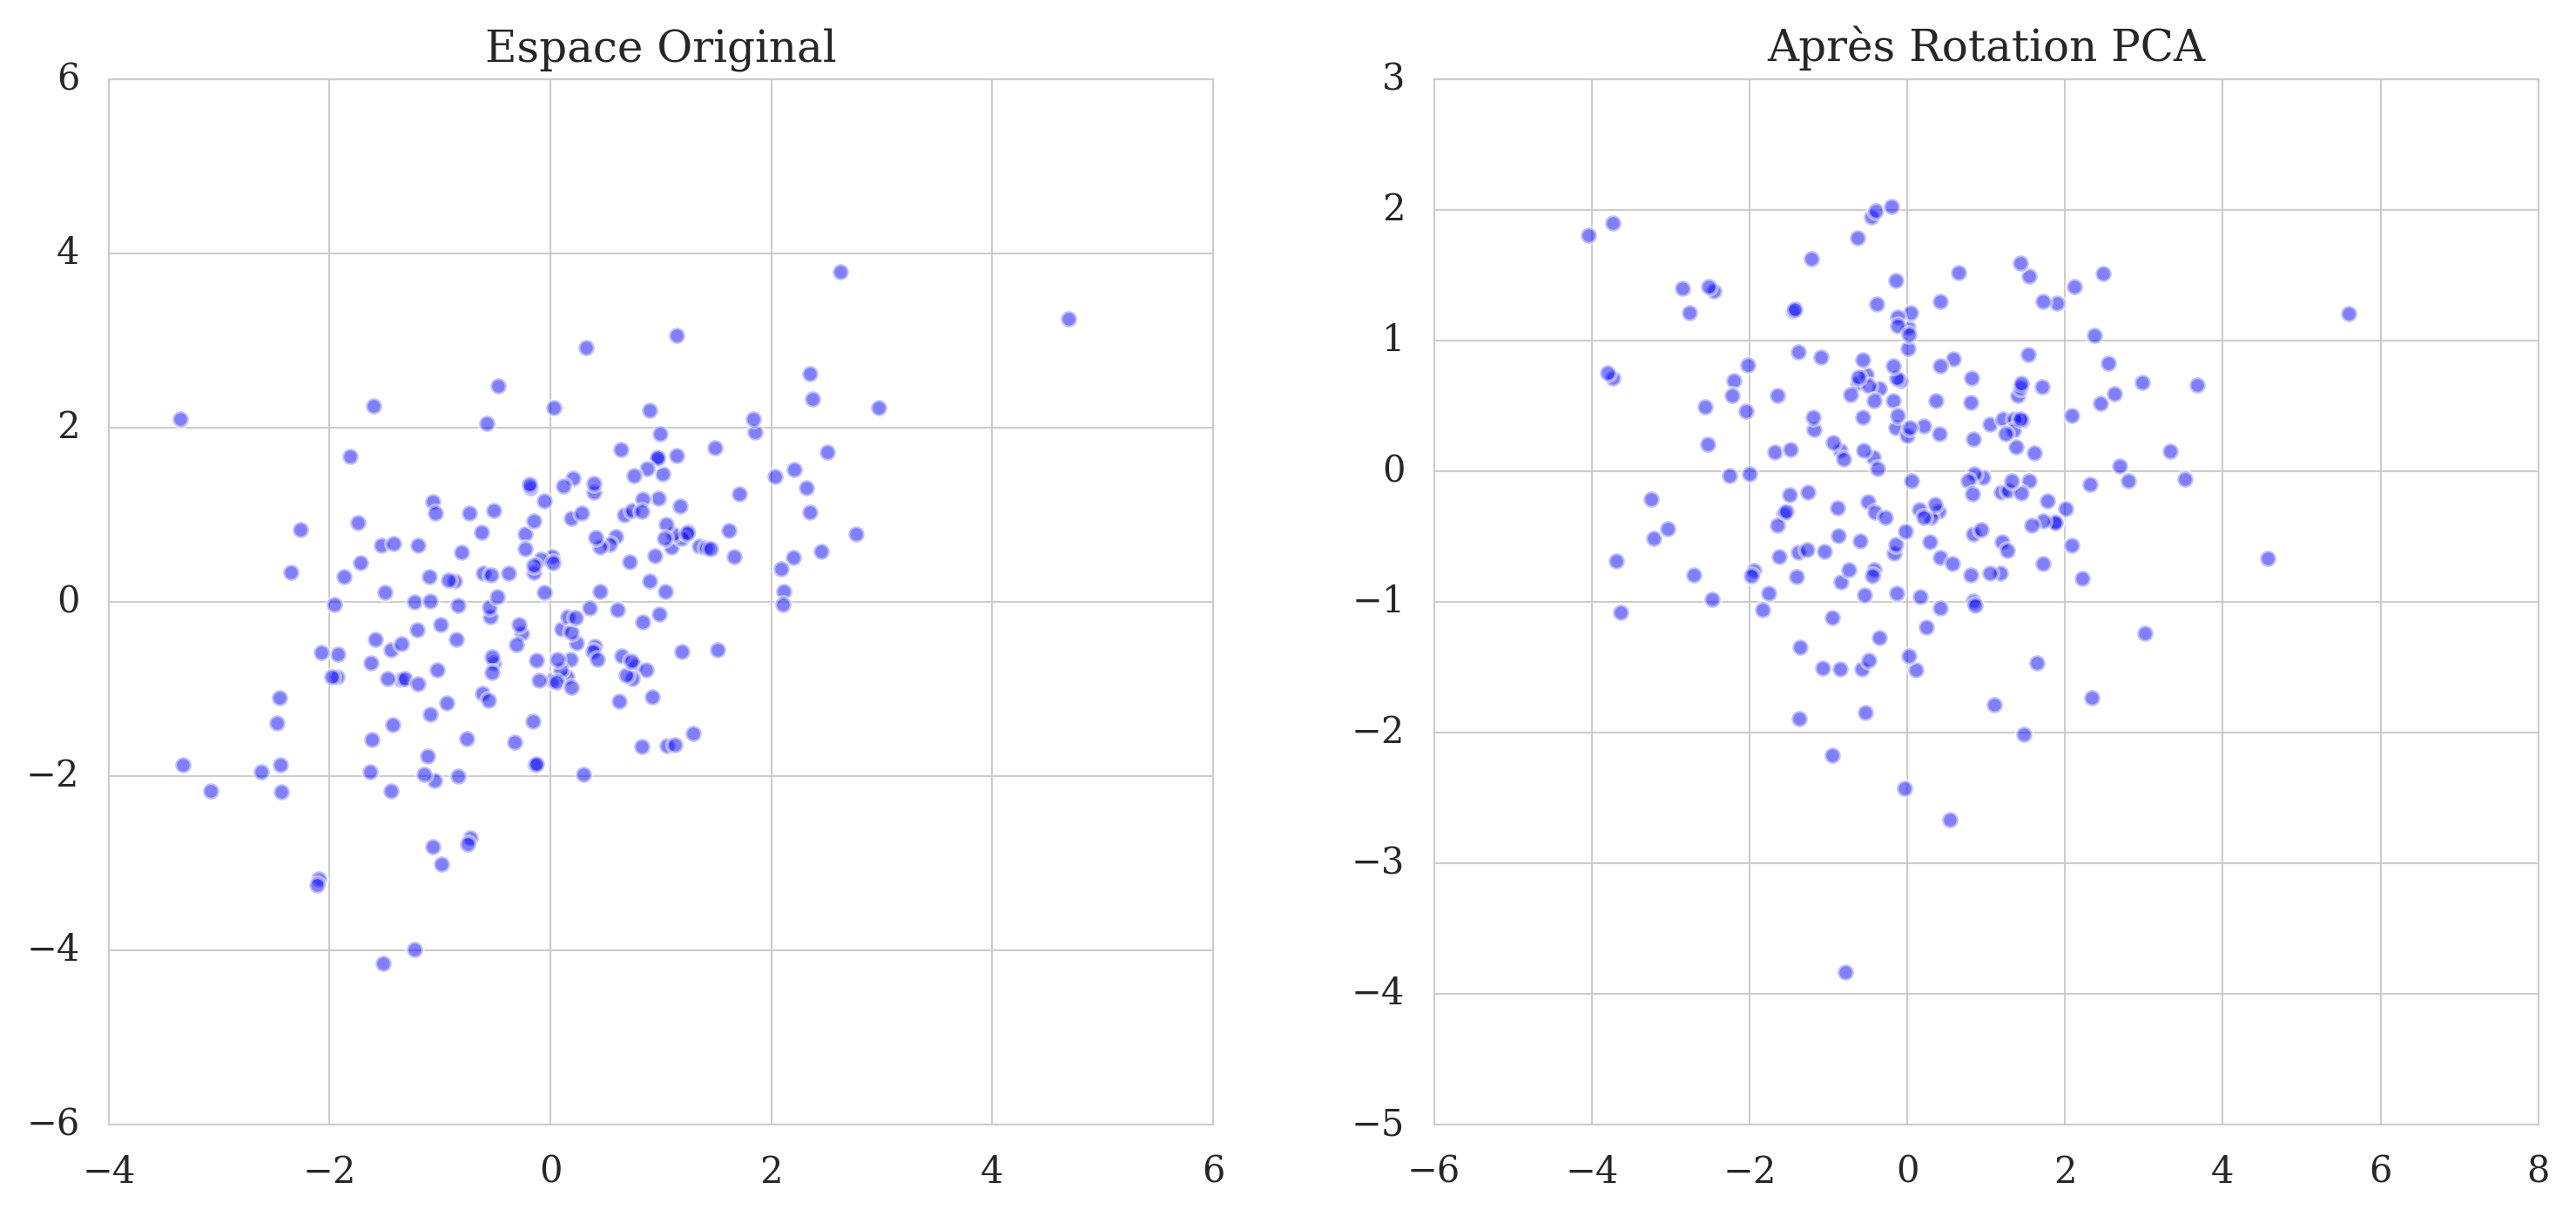
\includegraphics[width=0.8\textwidth]{pca_geometric.png}
\caption{L'ACP peut être vue comme une rotation rigide de l'espace des données.}
\end{figure}
\end{frame}

\section{Limitations de l'ACP classique}

\begin{frame}{Limitation : Linéarité}
L'ACP, de par sa nature linéaire, ne peut capturer que des relations linéaires entre les variables.

\begin{figure}
\centering
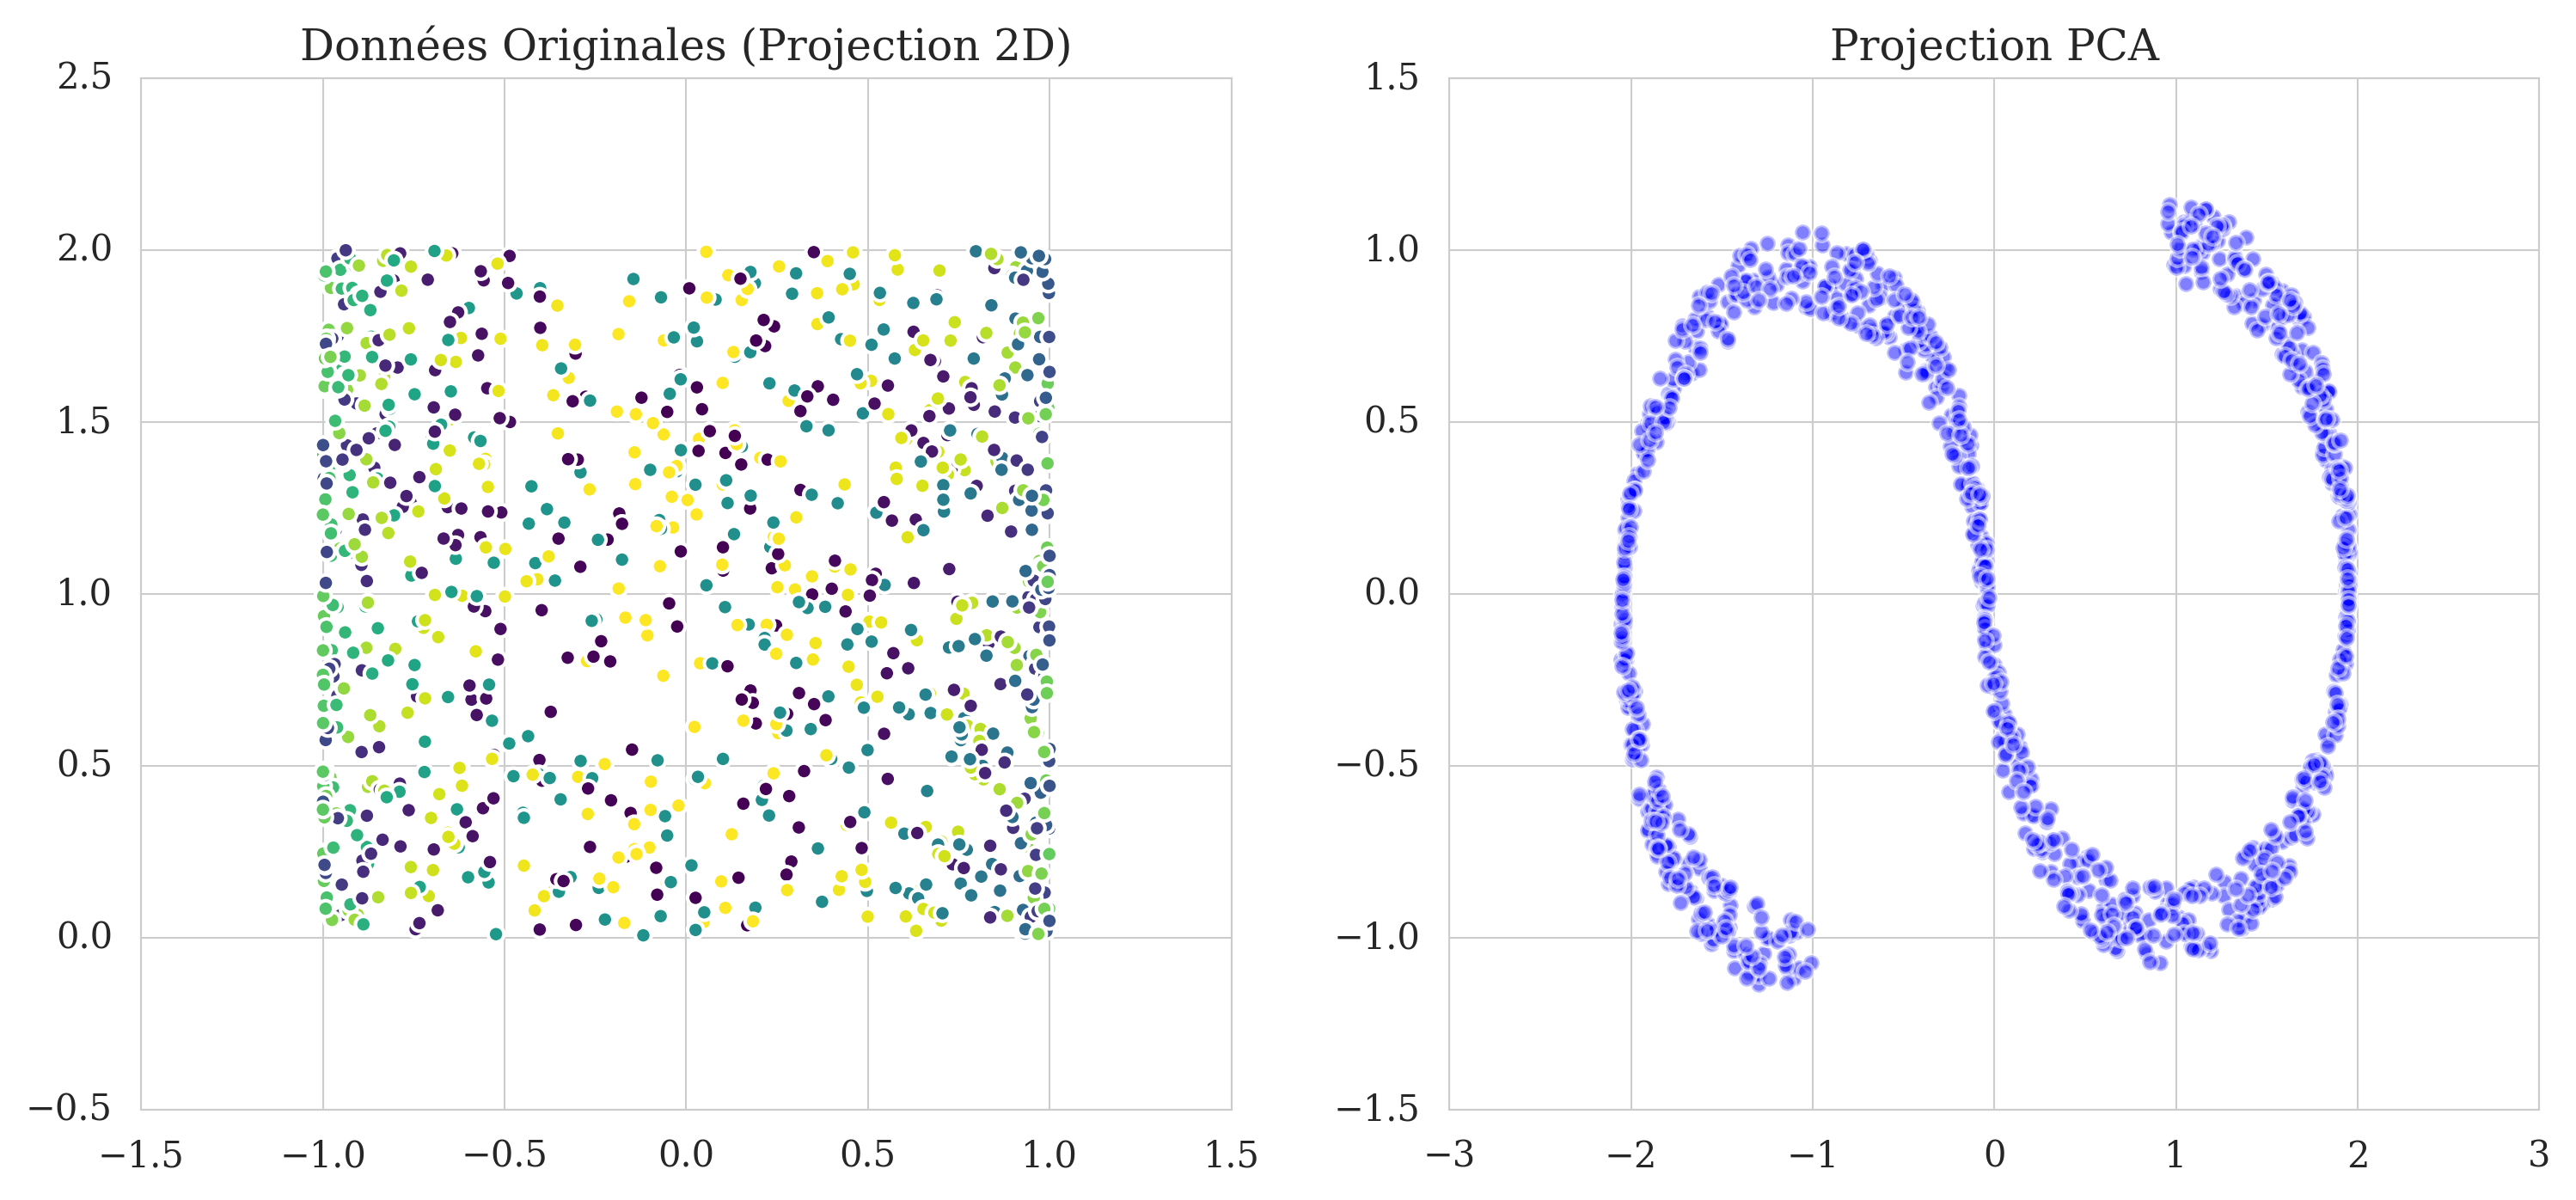
\includegraphics[width=0.7\textwidth]{nonlinear_pca_fail.png}
\caption{Données non linéaires pour lesquelles l'ACP échoue à restituer la structure (elle ne peut \og dérouler \fg{} la spirale).}
\end{figure}

\textit{Exemple : considérez des données disposées en spirale en 2D. L'ACP ne pourra pas dérouler cette spirale car elle se limite aux transformations linéaires.}
\end{frame}

\begin{frame}{Limitation : Sensibilité aux valeurs aberrantes}
L'ACP classique est très sensible aux \emph{outliers}, car elle se base sur la variance qui est elle-même sensible aux valeurs extrêmes.

\begin{figure}
\centering
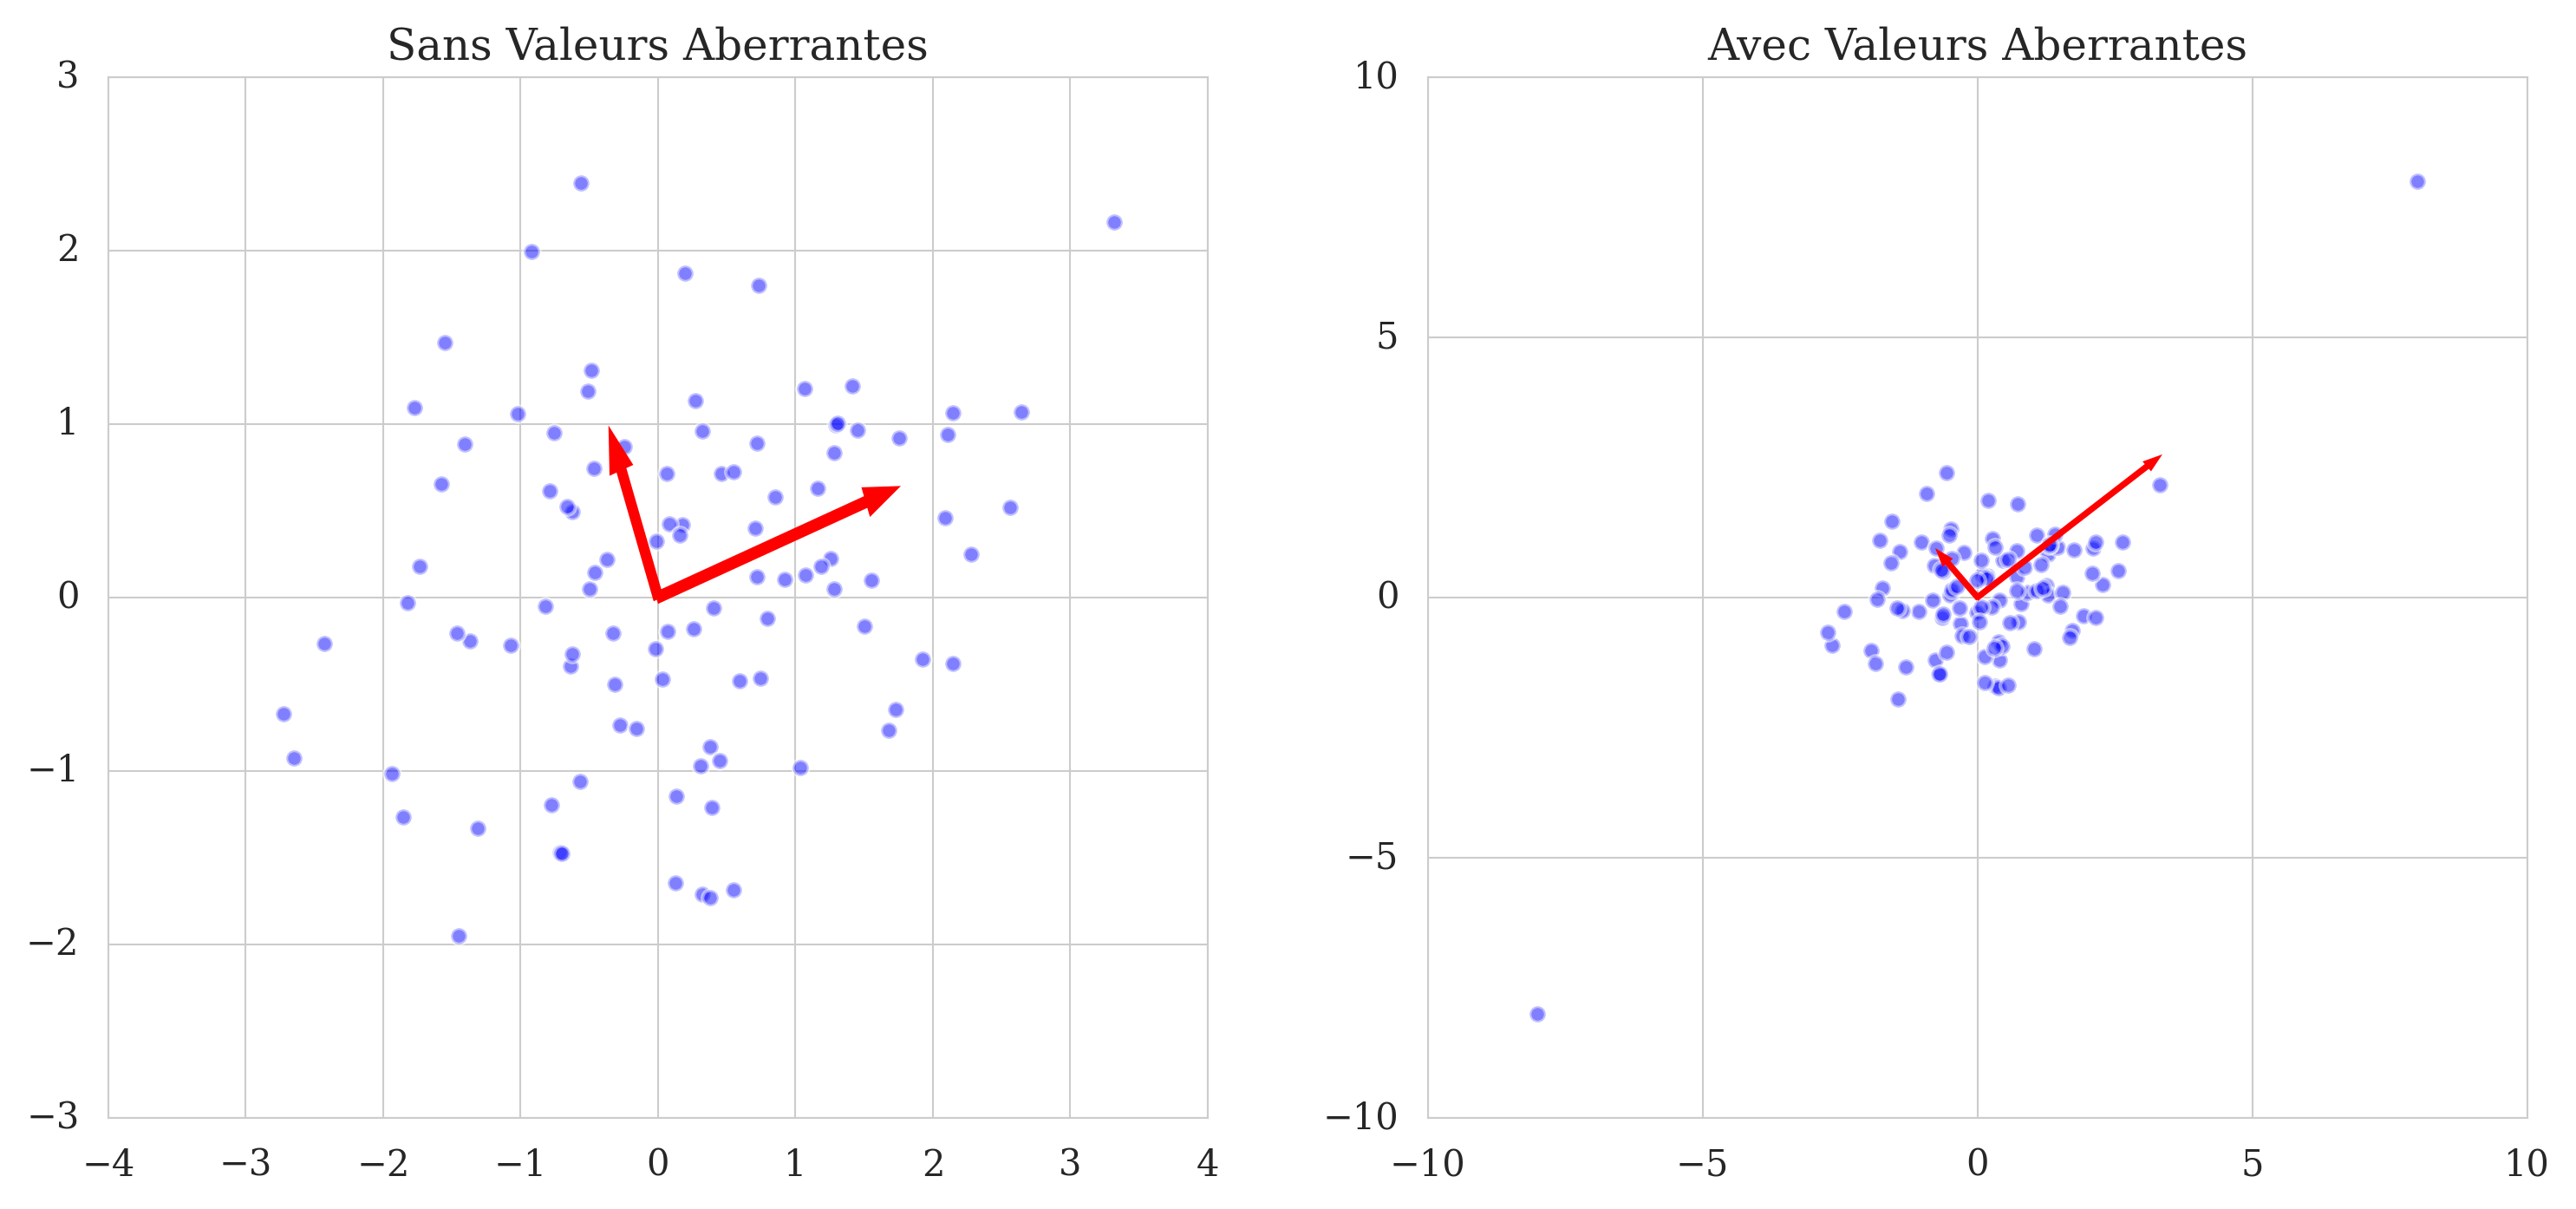
\includegraphics[width=0.7\textwidth]{outliers_impact.png}
\caption{Impact de valeurs aberrantes (points rouges) sur les composantes principales. Un seul \emph{outlier} peut fortement faire pivoter les axes principaux.}
\end{figure}

\textit{Exemple : dans un jeu de données financières, un seul point aberrant (p.~ex. un crash boursier) peut complètement modifier l'orientation des composantes principales.}
\end{frame}

\begin{frame}{Limitation : Hypothèse de normalité}
L'ACP suppose implicitement que les données suivent une distribution normale multivariée, ce qui n'est pas toujours le cas en pratique.

\textit{Exemple : pour des données de consommation électrique, les distributions sont souvent asymétriques avec des pics aux heures de pointe, violant l'hypothèse de normalité.}
\end{frame}

\begin{frame}{Limitation : Perte d'interprétabilité}
Les composantes principales sont des combinaisons linéaires de toutes les variables initiales, ce qui peut rendre leur interprétation difficile.

\textit{Exemple : dans une étude médicale avec 100 variables mesurées, chaque composante principale peut impliquer toutes ces variables avec des coefficients non nuls, rendant l'interprétation clinique complexe.}
\end{frame}

\begin{frame}{Solutions alternatives}
\begin{itemize}
    \item \textbf{Kernel PCA} : introduit des transformations non linéaires (noyaux) pour capturer des relations complexes.
    \item \textbf{Robust PCA} : intègre des méthodes robustes pour réduire l'influence des valeurs aberrantes.
    \item \textbf{Sparse PCA} : impose de la parcimonie pour obtenir des composantes plus facilement interprétables (quelques variables contributrices principales).
    \item \textbf{Probabilistic PCA} : formule l'ACP dans un cadre probabiliste pour tenir compte de l'incertitude (suppose un modèle statistique sous-jacent).
\end{itemize}
\end{frame}

\begin{frame}{Résumé des limitations et solutions}
\footnotesize
\begin{center}
\begin{tabular}{|l|l|l|}
\hline
\textbf{Limitation} & \textbf{Impact} & \textbf{Solution} \\
\hline
Linéarité & Relations non linéaires mal captées & Kernel PCA \\
\hline
Outliers & Distorsion des composantes & Robust PCA \\
\hline
Interprétabilité & Difficile d'analyse & Sparse PCA \\
\hline
Normalité & Biais si données non gaussiennes & Probabilistic PCA \\
\hline
\end{tabular}
\end{center}

\vspace{0.2cm}
\scriptsize{\textit{NB : Comprendre ces limitations est essentiel pour choisir la variante d'ACP appropriée selon le contexte et la nature des données.}}
\end{frame}

\section{Matériel et méthodes}

\begin{frame}{Matériel et méthodes}
\begin{itemize}
  \item \textbf{Données :} une image de test haute résolution ($512\times512$ pixels, en niveaux de gris) issue d’une banque libre, et la base de visages ORL (400 images $64\times64$, en niveaux de gris).
  \item \textbf{Prétraitement :} centrage systématique des données (moyenne nulle par variable). Conversion des images en niveaux de gris et vectorisation. Normalisation supplémentaire (variance unitaire ou mise à l’échelle $[0,1]$) appliquée si nécessaire pour homogénéiser l’échelle.
  \item \textbf{Outils :} langage Python (v3.x) avec bibliothèques NumPy (calcul matriciel, SVD), SciPy/\textit{scikit-learn} (algorithmes d’ACP), Matplotlib (visualisation), \textit{scikit-image} (lecture d’images, calcul de SSIM).
  \item \textbf{Environnement :} Notebooks Jupyter (distribution Anaconda) sous Windows 10.
\end{itemize}
\end{frame}

\section{Application pratique de l'ACP}

\begin{frame}{Réduction de dimension et qualité visuelle (I)}
L’ACP permet de projeter une image haute définition dans un espace latent de dimension beaucoup plus faible tout en préservant l’essentiel de l’information perceptuelle.

\begin{figure}
  \centering
  \begin{subfigure}{0.18\textwidth}
    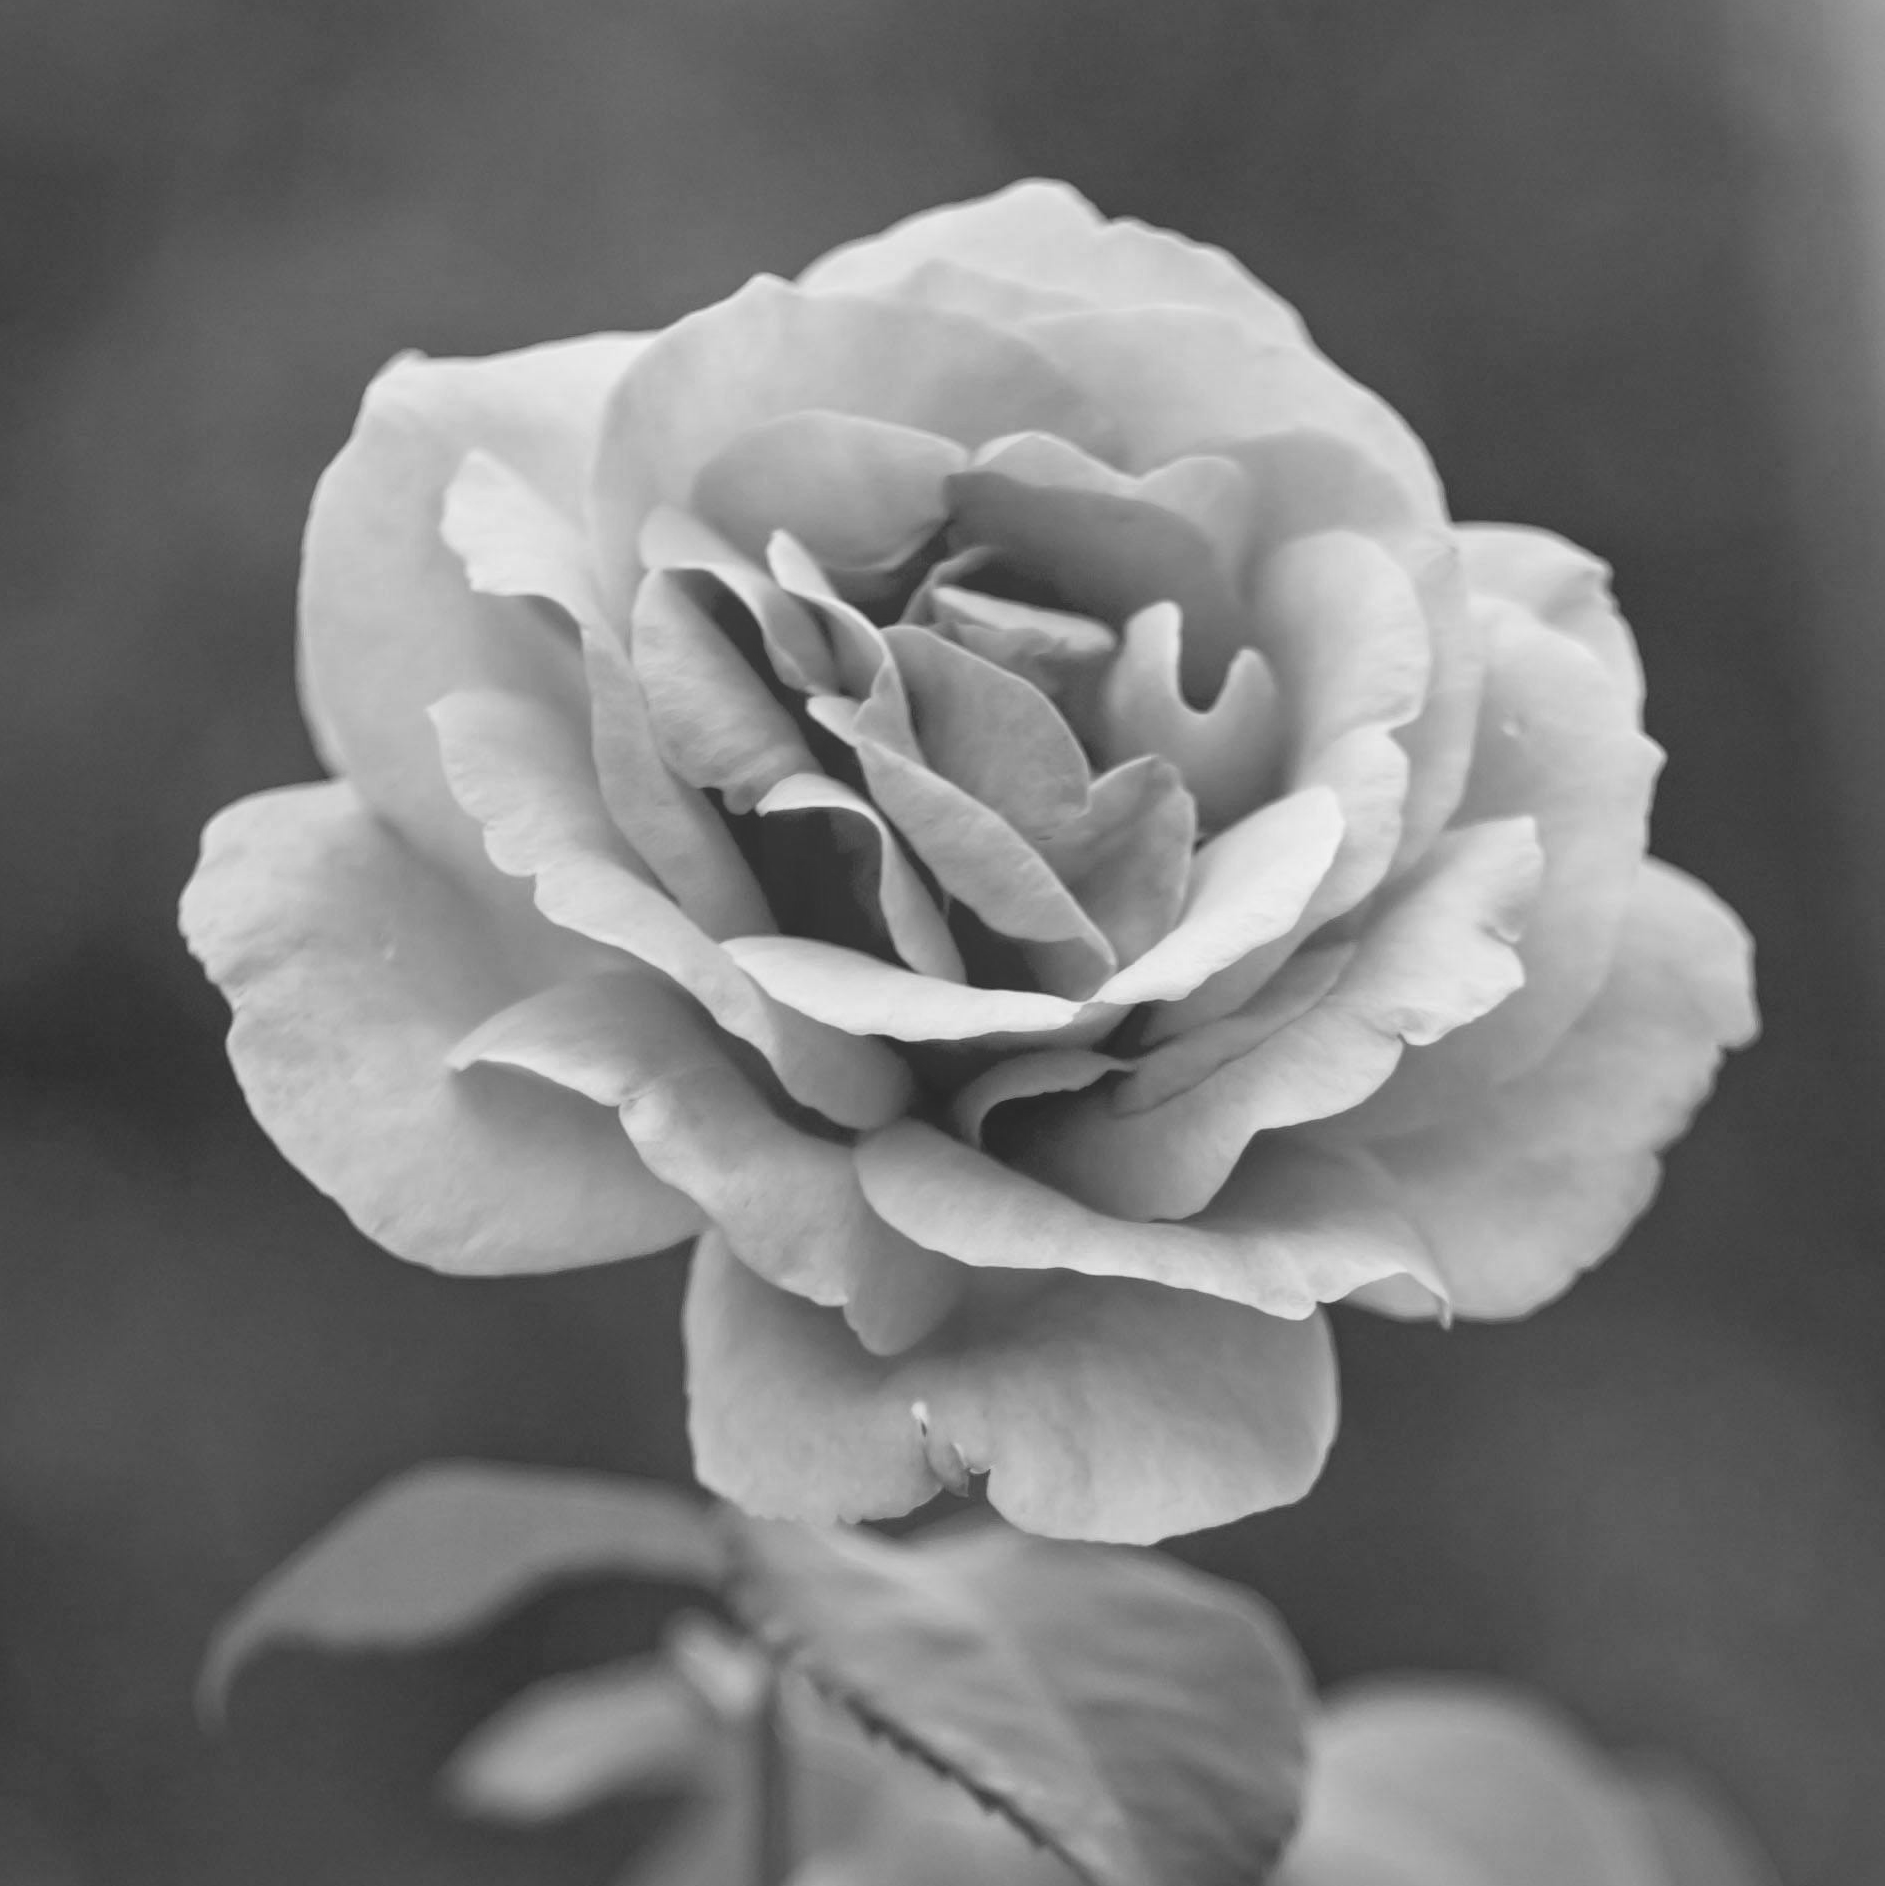
\includegraphics[width=\linewidth]{images/original.png}
    \caption*{Original}
  \end{subfigure}\hfill
  \begin{subfigure}{0.18\textwidth}
    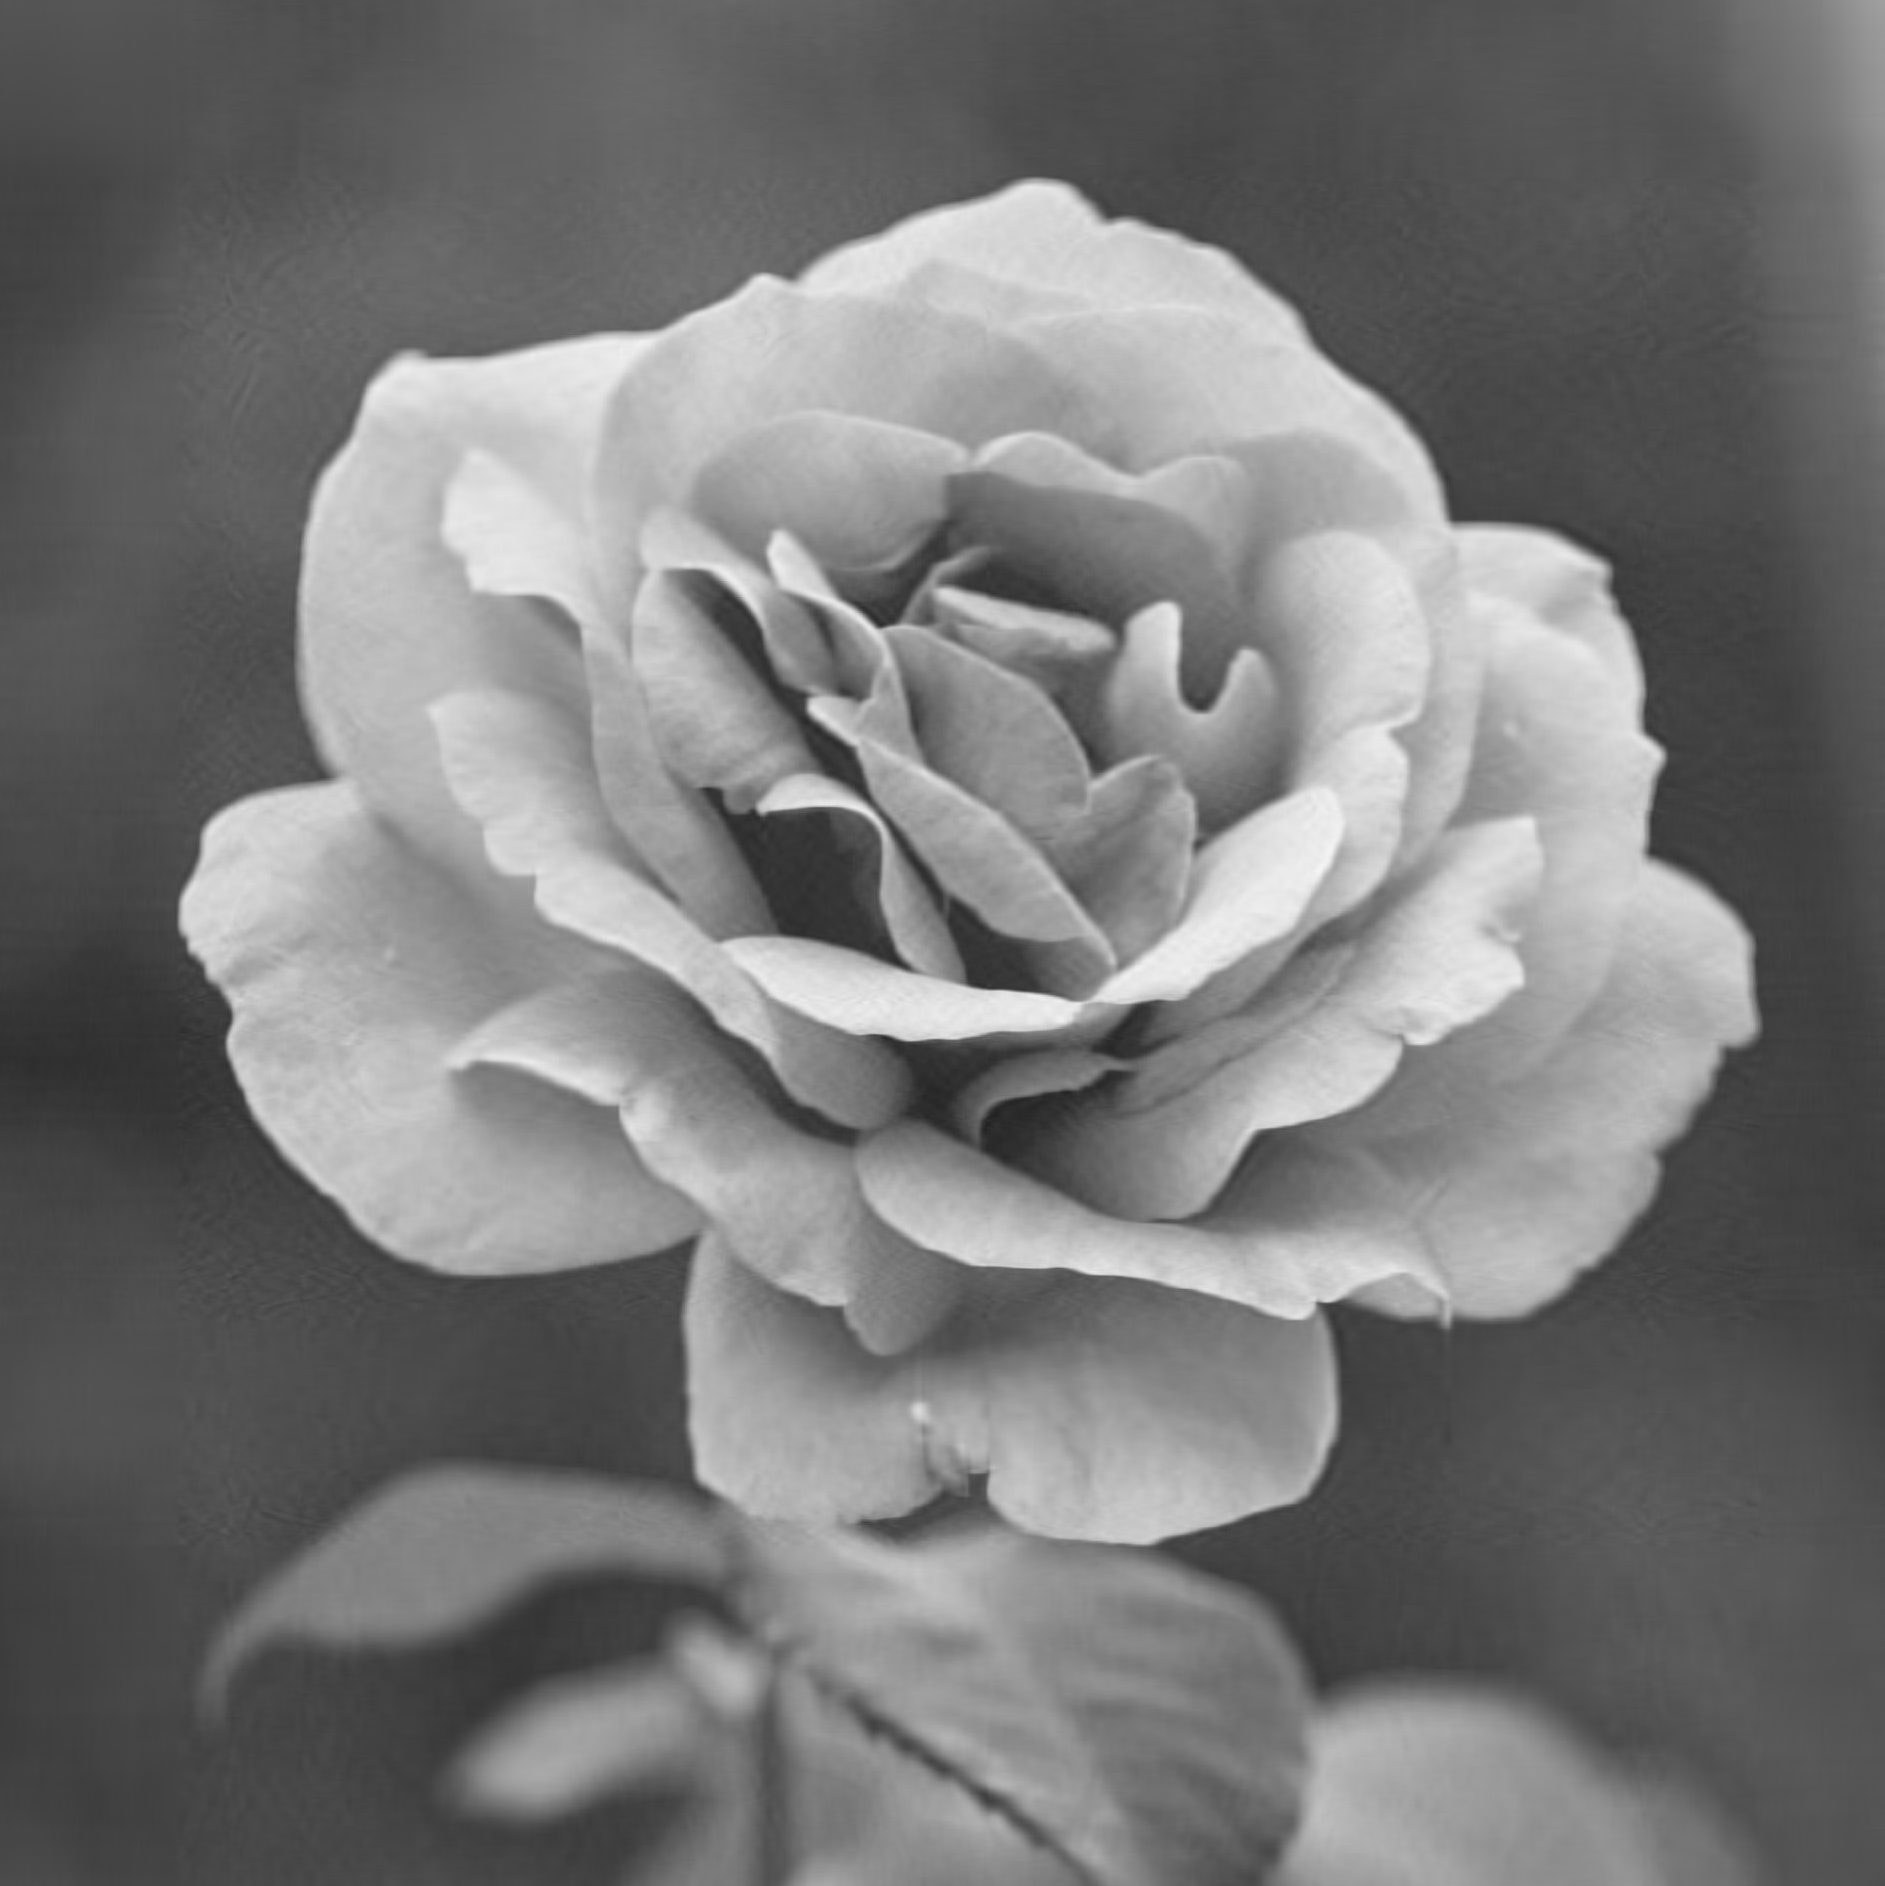
\includegraphics[width=\linewidth]{images/pca_100.png}
    \caption*{100 composantes}
  \end{subfigure}\hfill
  \begin{subfigure}{0.18\textwidth}
    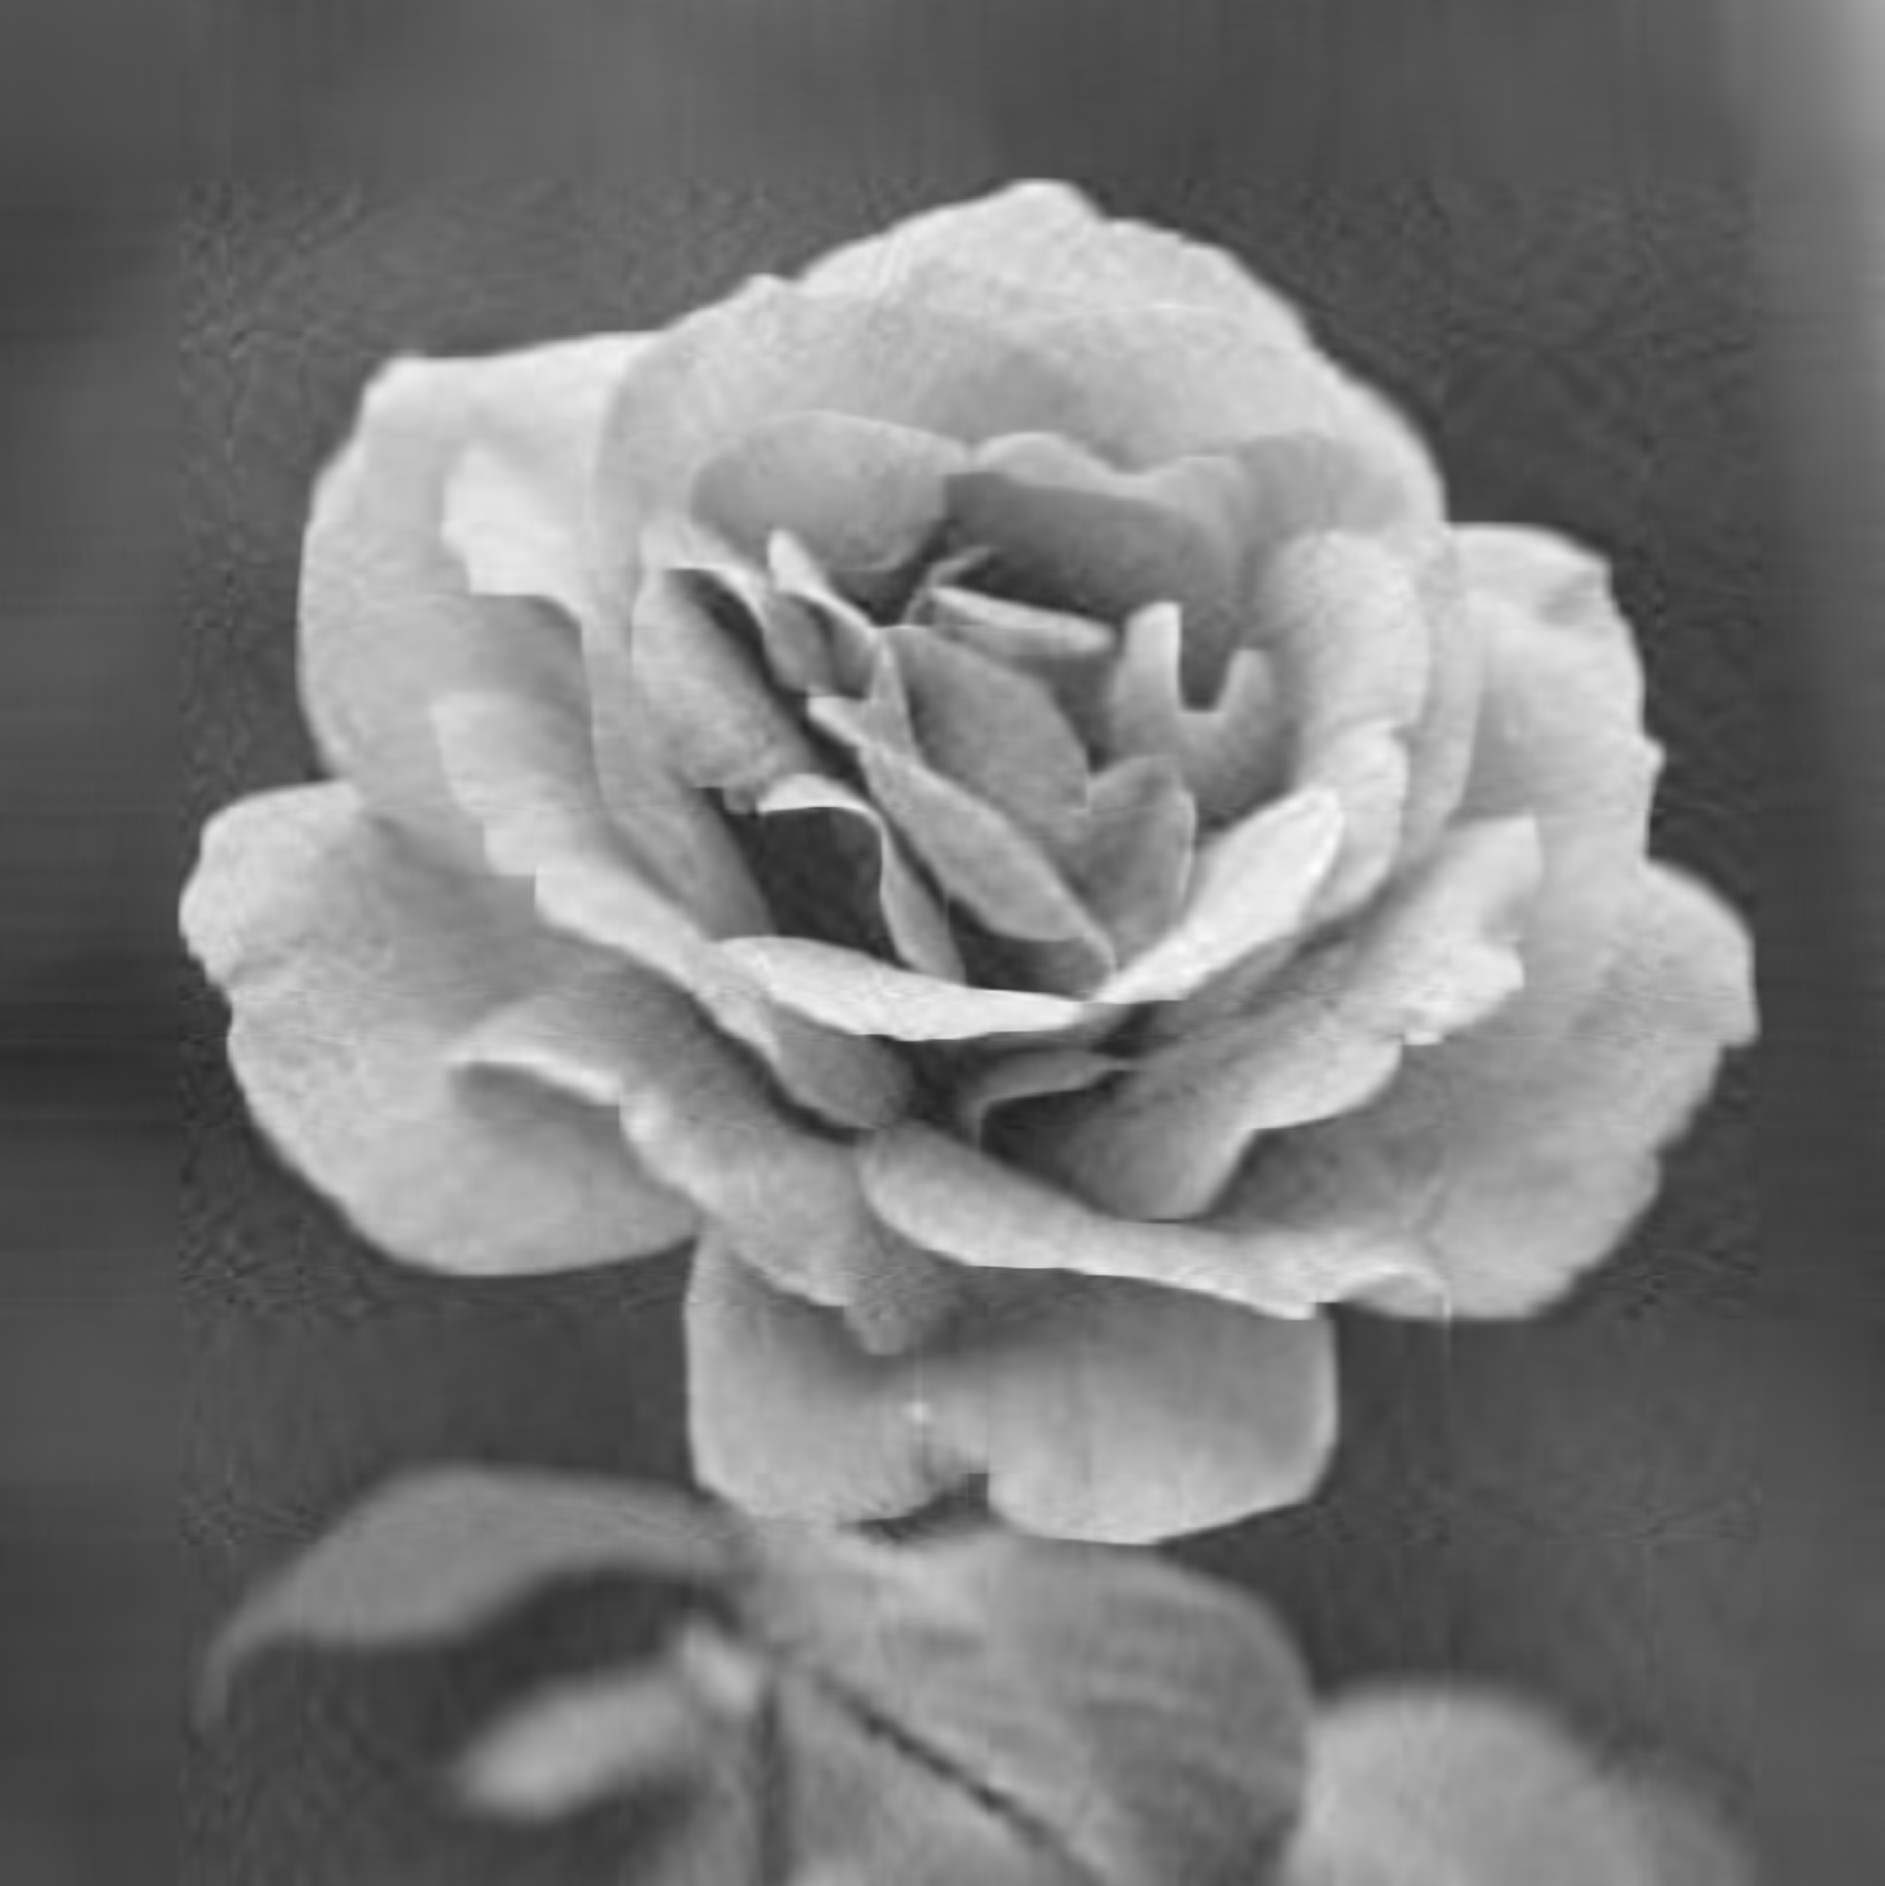
\includegraphics[width=\linewidth]{images/pca_50.png}
    \caption*{50 composantes}
  \end{subfigure}\hfill
  \begin{subfigure}{0.18\textwidth}
    
\includegraphics[width=\linewidth]{images/pca_25.png}
    \caption*{25 composantes}
  \end{subfigure}\hfill
  \begin{subfigure}{0.18\textwidth}
    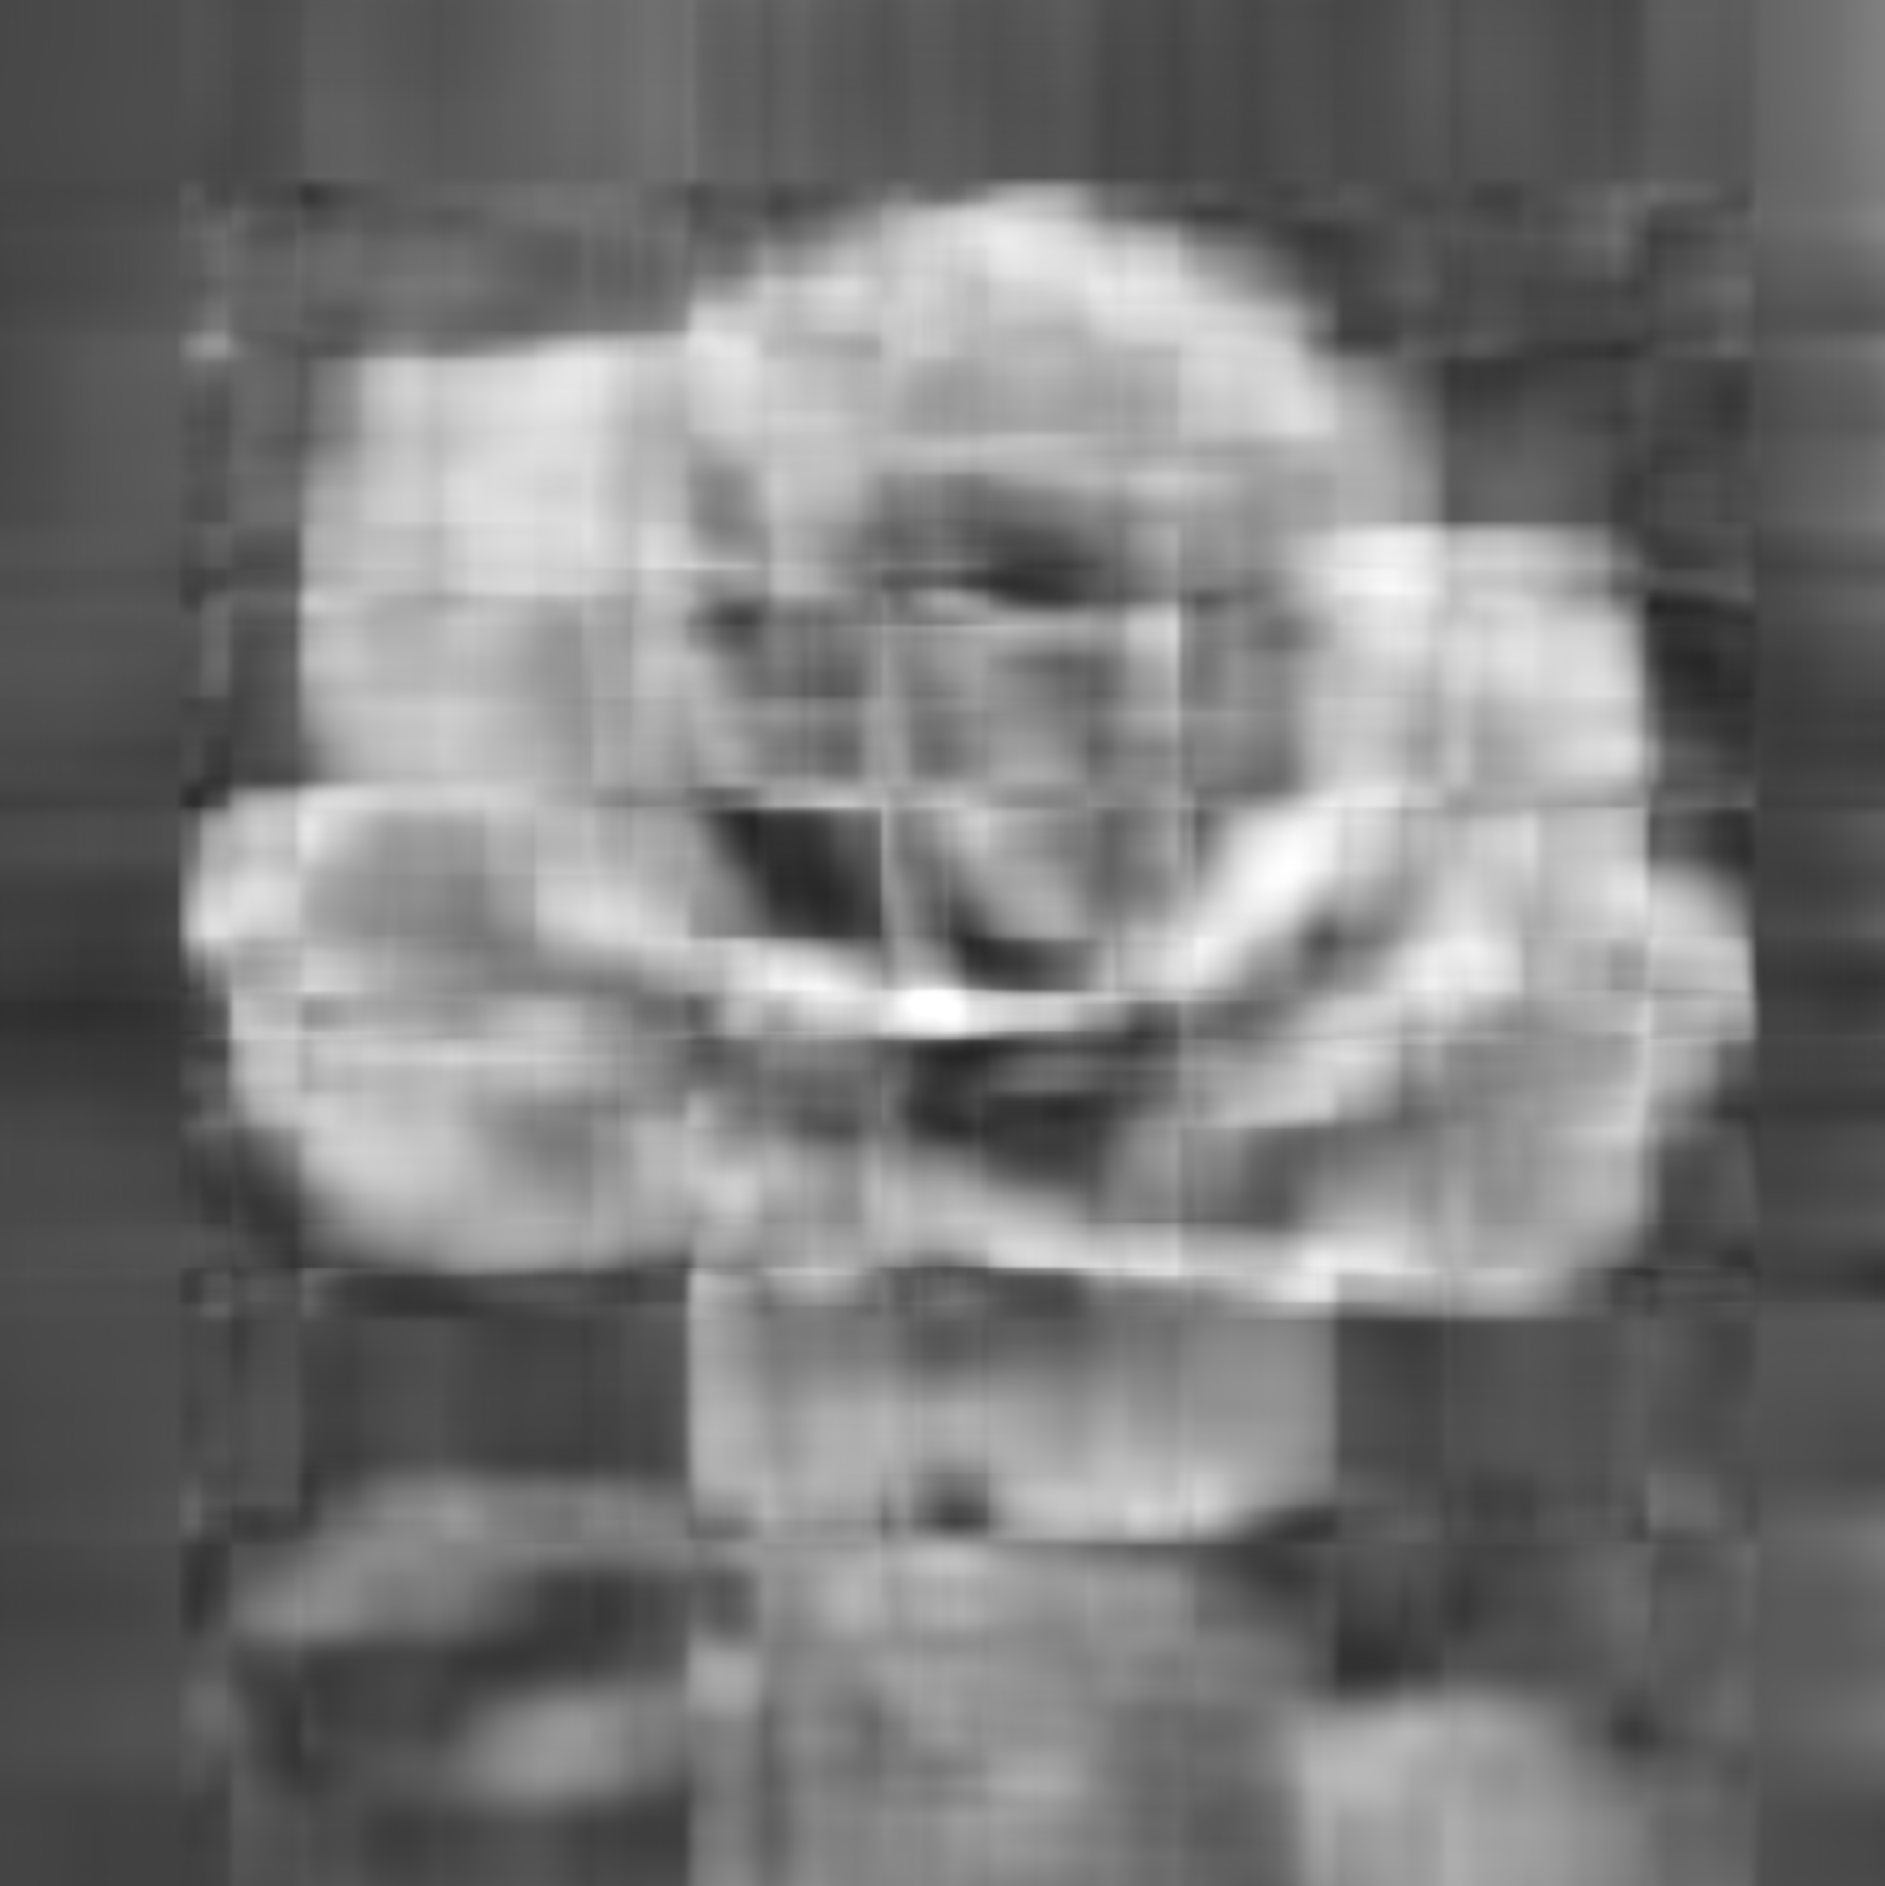
\includegraphics[width=\linewidth]{images/pca_10.png}
    \caption*{10 composantes}
  \end{subfigure}
  \caption{Effet du nombre de composantes principales $k$ sur la qualité visuelle.}
\end{figure}

On observe une dégradation graduelle : de l’image originale ($n$ dimensions) à des reconstructions avec $k=100$, $50$, $25$ et $10$ composantes principales.
\end{frame}

\begin{frame}{Réduction de dimension et qualité visuelle (II)}
\begin{figure}
  \centering
  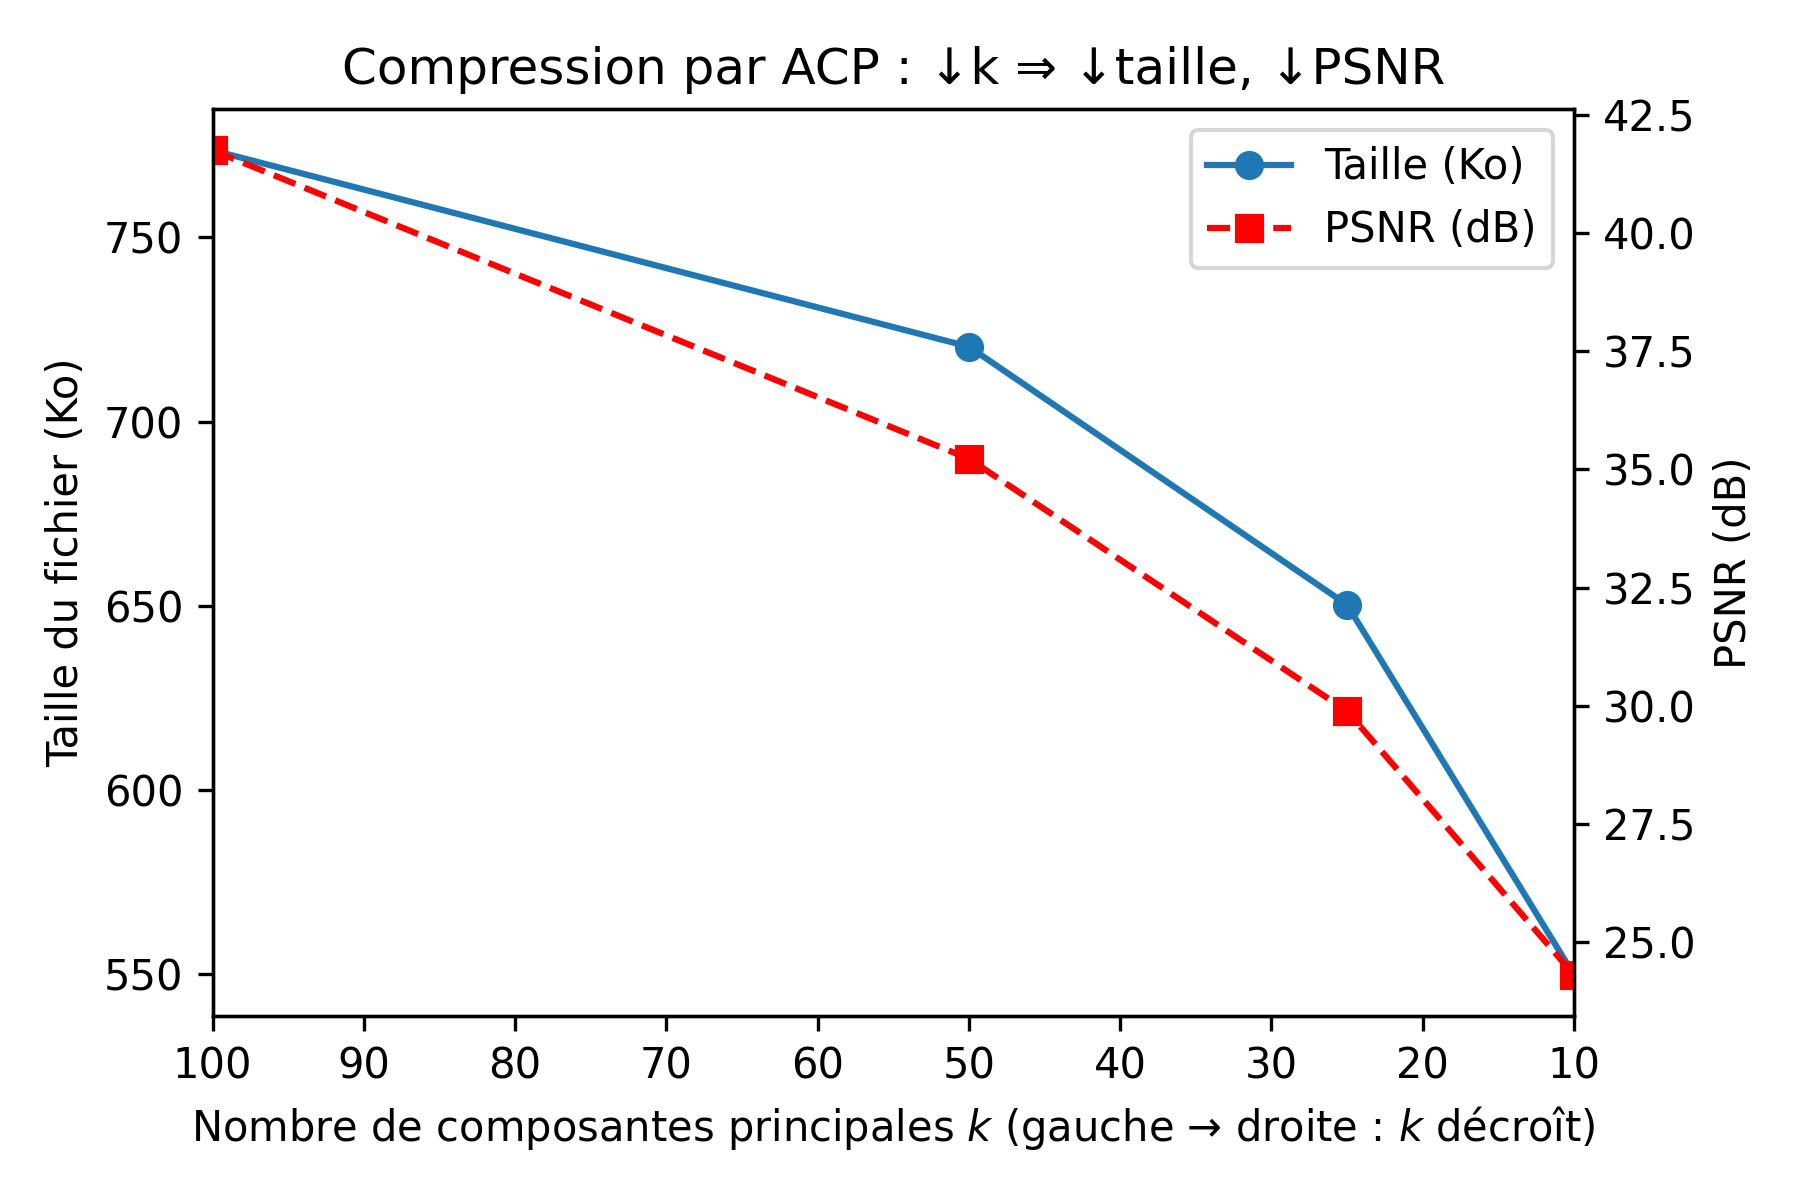
\includegraphics[width=0.85\textwidth]{images/pca_storage_vs_quality.png}
  \caption{Relation entre le nombre de composantes $k$, la taille du fichier (Ko) et la qualité de reconstruction (PSNR en dB).}
\end{figure}

%On remarque qu'entre $k=25$ et $k=50$, le gain en qualité devient marginal alors que la taille du fichier double.
\end{frame}

\begin{frame}{Eigenfaces : Méthode de Reconnaissance Faciale}
\begin{itemize}
  \item On dispose d’un ensemble d’images de visages alignées et centrées.
  \item Chaque image $I$ est convertie en vecteur de pixels, puis centrée : 
        \[
          I_{\text{centré}} = I - I_{\text{mean}}.
        \]
  \item L’ACP est appliquée à la matrice de données de dimension $n \times p$ (images × pixels).
\end{itemize}
\end{frame}

\begin{frame}{Rôle central de l’ACP dans Eigenfaces}
\small
\begin{itemize}
  \item Soit un ensemble de $n$ images vectorisées $I_1,\dots,I_n\in\mathbb{R}^p$, et leur moyenne
    \[
      I_{\rm mean} = \frac1n\sum_{i=1}^n I_i.
    \]
  \item Définissons la matrice de données centrée
    \[
      X = \bigl[I_1 - I_{\rm mean},\;\dots,\;I_n - I_{\rm mean}\bigr]\in\mathbb{R}^{p\times n}.
    \]
  \item Tout visage $I$ s'encode alors par les coefficients
    \[
      z = W^{\top}(I - I_{\rm mean})\in\mathbb{R}^K,
    \]
    assurant :
    \begin{itemize}
      \item réduction de dimension : $p\to K\ll p$,
      \item filtrage du bruit : on supprime les composantes de faible variance,
      \item extraction des traits dominants : chaque $w_i$ capture une “direction” de variation.
    \end{itemize}
\end{itemize}
\end{frame}

\section{Résultats et Analyses}


\begin{frame}[t]{SSIM : principe et application à l’ACP}
\small
\begin{columns}[T,onlytextwidth]

\column{0.48\textwidth}
\textbf{1. Principe du SSIM}\\[0.4em]
{
  \setlength{\itemsep}{0.15em}
  \begin{itemize}
    \item \alert{Objectif :} quantifier la similarité \emph{perçue} entre deux images.
    \item Trois composantes locales (fenêtre $11\times11$) :
      \[
        \text{SSIM}=
          \underbrace{l(x,y)}_{\text{luminance}}\times
          \underbrace{c(x,y)}_{\text{contraste}}\times
          \underbrace{s(x,y)}_{\text{structure}}
      \]
      avec
      \[\begin{aligned}
        l&=\frac{2\mu_x\mu_y+C_1}{\mu_x^2+\mu_y^2+C_1}
        c&=\frac{2\sigma_x\sigma_y+C_2}{\sigma_x^2+\sigma_y^2+C_2}\\
        s&=\frac{\sigma_{xy}+C_3}{\sigma_x\sigma_y+C_3}
      \end{aligned}\]
    \item $\text{SSIM}\in[-1,1]$ : $1$ identique, $0$ aucune corrélation.
  \end{itemize}
}

\column{0.5\textwidth}
\textbf{2. Comment l’utiliser avec l’ACP ?}\\[0.4em]
{
  \setlength{\itemsep}{0.4em}
  \begin{enumerate}
    \item \textbf{Compression PCA}\\
          $\triangleright$ Réduire la dimension (images vectorisées).\\
          $\triangleright$ Reconstruire avec $k$ composantes.
    \item \textbf{Évaluation par SSIM}\\
          $\triangleright$ Calculer SSIM(img$_\text{réelle}$, img$_\text{reconst}$).\\
          $\triangleright$ Tracer SSIM vs.\ $k$ pour un compromis qualité/taille.
    \item \textbf{Sélection adaptative}\\
          Point où SSIM $<0.95$ pour fixer $k$.
    \item \textbf{Critère d’arrêt}\\
          Arrêter dès que $\Delta\text{SSIM} < \varepsilon$.
  \end{enumerate}
}

\end{columns}
\end{frame}



\begin{frame}[t,fragile]{Calcul de $\mu_x$ et $\mu_y$}
\small
\setlength{\itemsep}{0.35em}
\begin{itemize}
  \item \textbf{Fenêtre :} généralement $11\times11$ ou $8\times8$.
  \item \textbf{Filtre gaussien 2-D} ($\sigma\simeq1.5$) pour pondérer :
    \[
      \mu_x(i,j)=\sum_{u,v} w(u,v)\,X(i+u,j+v),\quad
      \mu_y(i,j)=\sum_{u,v} w(u,v)\,Y(i+u,j+v)
    \]
  \item \textbf{Implémentation rapide} : convolution ou \texttt{GaussianBlur}.
\end{itemize}

\vspace{0.2em}
\textit{Exemple Python (OpenCV)} :
\begin{verbatim}
mu_x = cv2.GaussianBlur(X, (11, 11), 1.5)
mu_y = cv2.GaussianBlur(Y, (11, 11), 1.5)
\end{verbatim}
\end{frame}


\begin{frame}[t]{Constantes $C_1, C_2, C_3$}
\small
\begin{block}{Formules générales}
\[
  C_1 = (K_1\,L)^2,\quad
  C_2 = (K_2\,L)^2,\quad
  C_3 = \frac{C_2}{2}
\]
\end{block}

\setlength{\itemsep}{0.4em}
\begin{itemize}
  \item $L$ : dynamique des intensités (8 bits $\to$ 255, flottant $\to$ 1).
  \item Paramètres conseillés : $K_1 = 0.01$, $K_2 = 0.03$.
  \item \textbf{Images 8 bits} ($L = 255$) :  
        $C_1 \approx 6.5025$, $C_2 \approx 58.5225$, $C_3 \approx 29.2612$.
  \item \textbf{Images normalisées} ($L = 1$) :  
        $C_1 = 1\times10^{-4}$, $C_2 = 9\times10^{-4}$, $C_3 = 4.5\times10^{-4}$.
\end{itemize}

\begin{alertblock}{À retenir}
$\mu_x,\,\mu_y$ : moyennes locales via un filtre gaussien.\\
$C_1,\,C_2,\,C_3$ : dérivés de la dynamique $L$ et de deux petits coefficients
$K_1$, $K_2$ pour stabiliser la division.\\
Toujours ajuster ces constantes à l’échelle choisie ($[0,255]$ ou $[0,1]$).
\end{alertblock}
\end{frame}




\begin{frame}{Évaluation quantitative}
\begin{center}
\small
\begin{tabular}{c|c|c|c}
$k$ & MSE & PSNR (dB) & SSIM \\
\hline
100 & 20 & 35.1 & 0.98 \\
50 & 65 & 30.2 & 0.95 \\
25 & 200 & 25.1 & 0.90 \\
10 & 650 & 20.0 & 0.80 \\
\end{tabular}
\end{center}
\vspace{0.2cm}
\footnotesize{Métriques de reconstruction de l'image test en fonction du nombre de composantes principales $k$.}
\end{frame}

\begin{frame}{Analyse des résultats}
\begin{itemize}
  \item La courbe du PSNR en fonction de $k$ présente un \textit{point de coude} : au-delà d’environ 25 composantes, les gains supplémentaires de PSNR deviennent très limités alors que la taille des données double (rendements décroissants).
  \item Le SSIM (indice de similarité structurelle) corrobore le PSNR : il demeure élevé ($\approx 0.95$) pour $k \ge 50$, puis chute drastiquement lorsque $k$ est trop faible (p.~ex. $0.80$ à $k=10$), traduisant une perte des structures perceptibles.
  \item La reconstruction par ACP surpasse une compression \og naïve\fg{} : en tant qu’approximation de rang-$k$ optimale minimisant l’erreur quadratique moyenne, l’ACP fournit un PSNR supérieur pour une même taille de données comparée à une réduction de résolution ou une sélection aléatoire de pixels.
\end{itemize}
\end{frame}

\section{Conclusion \& Perspectives}

\begin{frame}{Conclusion \& Perspectives}
\begin{itemize}
  \item \textbf{Bilan :} La mise en œuvre de l’ACP sur des images a démontré qu’une réduction drastique du nombre de variables (jusqu’à ~90\%) est possible sans altération majeure de la qualité visuelle. Les objectifs du projet ont été atteints : compréhension théorique, implémentation pratique et évaluation quantitative (PSNR et SSIM) ont permis de valider l’approche sur des cas concrets.
  \item \textbf{Limites :} L’ACP classique reste sensible aux données aberrantes et ne capture que les relations linéaires. Elle peut conduire à une perte d’interprétabilité des composantes. Ces aspects n’ont pas pu être pleinement traités dans ce travail.
  \item \textbf{Perspectives :} Affiner le choix du nombre optimal de composantes (critère du coude, validation croisée) et explorer d’autres méthodes de réduction de dimension. En particulier, des approches non linéaires comme t-SNE ou UMAP offriraient des visualisations plus fidèles de structures complexes.
\end{itemize}
\end{frame}

\begin{frame}{Répositoire GitHub}
\centering
\vspace{1em}
{\Huge \textbf{Testez-vous même}}

\vspace{2em}

\begin{minipage}{0.45\textwidth}
    \centering
    
\includegraphics[width=\linewidth]{GitHub-Logo-ee398b662d42.png} 
\end{minipage}
\hfill
\begin{minipage}{0.45\textwidth}
    \centering
    
\includegraphics[width=\linewidth]{qr-code.png} 
    \captionof{figure}{Code QR du Repo GitHub}
\end{minipage}

\end{frame}

\begin{frame}[allowframebreaks]{Bibliographie}
\tiny
\begin{thebibliography}{9}
\bibitem{Pearson1901} Pearson, K. (1901). \textit{L'analyse des données}. Journal de Statistique.
\bibitem{Hotelling1933} Hotelling, H. (1933). Analysis of a complex of statistical variables into principal components. \textit{Journal of Educational Psychology}.
\bibitem{Jolliffe2002} Jolliffe, I.~T. (2002). \textit{Principal Component Analysis}. Springer.
\bibitem{Bishop2006} Bishop, C.~M. (2006). \textit{Pattern Recognition and Machine Learning}. Springer.
\bibitem{Scholkopf1998} Schölkopf, B., et al. (1998). Nonlinear Component Analysis as a Kernel Eigenvalue Problem. \textit{Neural Computation}.
\end{thebibliography}
\end{frame}

\begin{frame}[t,fragile]{Webographie}
\footnotesize
\begin{itemize}
    \item \url{https://scikit-learn.org/stable/modules/decomposition.html#pca} -- Documentation \textit{scikit-learn} sur l'ACP.
    \item \url{https://stats.stackexchange.com/questions/2691/making-sense-of-principal-component-analysis} -- Discussion approfondie sur l'ACP.
    \item \url{https://setosa.io/ev/principal-component-analysis/} -- Visualisation interactive de l'ACP.
    \item \url{https://www.cs.otago.ac.nz/cosc453/student_tutorials/principal_components.pdf} -- Tutoriel complet sur l'ACP.
    \item \url{https://www.kaggle.com/code/arthurtok/interactive-intro-to-dimensionality-reduction} -- Exemples pratiques d'ACP.
\end{itemize}
\end{frame}


\begin{frame}{Webographie (suite)}
\footnotesize
\begin{itemize}
    \item \url{https://www.datasciencecentral.com/principal-component-analysis-for-dimensionality-reduction/} -- Applications en data science.
    \item \url{https://mathworld.wolfram.com/PrincipalComponentAnalysis.html} -- Aspects mathématiques détaillés.
    \item \url{https://towardsdatascience.com/a-complete-guide-to-principal-component-analysis-pca-in-machine-learning-664f34fc6a27} -- Guide complet sur l'ACP.
    \item \url{https://en.wikipedia.org/wiki/Principal_component_analysis} -- Article Wikipedia détaillé.
    \item \url{https://www.youtube.com/watch?v=FgakZw6K1QQ} -- Vidéo explicative sur l'ACP.
\end{itemize}
\end{frame}

\section{Annexes}

\begin{frame}[t,fragile]{Extrait de code Python – ACP}
\lstset{
  language=Python,
  basicstyle=\ttfamily\scriptsize,
  inputencoding=utf8,
  extendedchars=true,
  literate={é}{{\'e}}1 {è}{{\`e}}1 {à}{{\`a}}1 {ù}{{\`u}}1
           {â}{{\^a}}1 {ê}{{\^e}}1 {î}{{\^i}}1 {ô}{{\^o}}1 {û}{{\^u}}1
}
\begin{lstlisting}[inputencoding=utf8]
import imageio
import numpy as np
# Chargement de l'image en niveau de gris
img = imageio.imread('images/original.png', as_gray=True)
# Décomposition SVD de l'image en composantes principales
U, S, Vt = np.linalg.svd(img, full_matrices=False)
k = 50  # nombre de composantes retenues
# Reconstruction approchée de l'image avec k composantes
img_rec = U[:, :k] @ np.diag(S[:k]) @ Vt[:k, :]
# Calcul de l'erreur quadratique moyenne (MSE) et du PSNR
mse = np.mean((img - img_rec)**2)
psnr = 10 * np.log10((255**2) / mse)
print(f"PSNR = {psnr:.2f} dB")
\end{lstlisting}
\end{frame}



\begin{frame}{Paramètres d'exécution}
\begin{itemize}
  \item \textbf{Machine :} PC portable sous MacOS, CPU Intel Core i9, 32~Go de RAM.
  \item \textbf{Environnement :} Anaconda Python 3.10, exécution du code dans des scripts sur VsCode.
  \item \textbf{Bibliothèques :} NumPy 1.21, SciPy 1.7, scikit-learn 1.2, Matplotlib 3.4, scikit-image 0.18.
  \item \textbf{Temps de calcul :} de l’ordre de la seconde pour les cas étudiés (p.~ex. $\approx$0.2~s pour une image $512\times512$, $\approx$1~s pour 400 matrice $64\times64$, sur CPU).
\end{itemize}
\end{frame}

\end{document}
